\documentclass[USenglish]{ifimaster}

\usepackage[export]{adjustbox}
\usepackage[utf8]{inputenc}
\usepackage{ifimasterforside}
\usepackage{graphicx}
\usepackage{subfig}
\usepackage{floatrow}
\usepackage{rotating}
\usepackage{pdflscape}

\usepackage[acronym, toc]{glossaries}
\usepackage[toc,page]{appendix}

\usepackage[backend=biber,sorting=none]{biblatex}
\usepackage{listings}

\usepackage{tabularx}
\usepackage{cleveref}

% For listings
\usepackage{bera}
\usepackage{listings}
\usepackage{xcolor}
\colorlet{punct}{red!60!black}
\definecolor{background}{HTML}{EEEEEE}
\definecolor{delim}{RGB}{20,105,176}
\colorlet{numb}{magenta!60!black}
\lstdefinelanguage{json}{
    basicstyle=\normalfont\ttfamily,
    numbers=left,
    numberstyle=\scriptsize,
    stepnumber=1,
    numbersep=8pt,
    showstringspaces=false,
    breaklines=true,
    frame=lines,
    backgroundcolor=\color{background},
    literate=
     *{0}{{{\color{numb}0}}}{1}
      {1}{{{\color{numb}1}}}{1}
      {2}{{{\color{numb}2}}}{1}
      {3}{{{\color{numb}3}}}{1}
      {4}{{{\color{numb}4}}}{1}
      {5}{{{\color{numb}5}}}{1}
      {6}{{{\color{numb}6}}}{1}
      {7}{{{\color{numb}7}}}{1}
      {8}{{{\color{numb}8}}}{1}
      {9}{{{\color{numb}9}}}{1}
      {:}{{{\color{punct}{:}}}}{1}
      {,}{{{\color{punct}{,}}}}{1}
      {\{}{{{\color{delim}{\{}}}}{1}
      {\}}{{{\color{delim}{\}}}}}{1}
      {[}{{{\color{delim}{[}}}}{1}
      {]}{{{\color{delim}{]}}}}{1},
}

\definecolor{pblue}{rgb}{0.13,0.13,1}
\definecolor{pgreen}{rgb}{0,0.5,0}
\definecolor{pred}{rgb}{0.9,0,0}
\definecolor{pgrey}{rgb}{0.46,0.45,0.48}
\lstset{language=Java,
  showspaces=false,
  showtabs=false,
  breaklines=true,
  showstringspaces=false,
  breakatwhitespace=true,
  commentstyle=\color{pgreen},
  keywordstyle=\color{pblue},
  stringstyle=\color{pred},
  basicstyle=\ttfamily,
  moredelim=[il][\textcolor{pgrey}]{$$},
  moredelim=[is][\textcolor{pgrey}]{\%\%}{\%\%}
}


\makeglossaries

% Acronyms
\newacronym{acm}{ACM}{Agile Computing Middleware}
\newacronym{afro}{AFRO}{Adaption Framework foR Web Services prOvision}
\newacronym{amqp}{AMQP}{Advanced Message Queuing Protocol}
\newacronym{api}{API}{Application Program Interface}
\newacronym{coap}{CoAP}{The Constrained Application Protocol}
\newacronym{cnr}{CNR}{Combat Net Radio}
\newacronym{cots}{COTS}{Commercial off-the-shelf}
\newacronym{dsproxy}{DSProxy}{Delay and disruption tolerant SOAP Proxy}
\newacronym{dil}{DIL}{Disconnected, Intermittent and Limited}
\newacronym{edge}{EDGE}{Enhanced Data rates for GSM Evolution}
\newacronym{efx}{EFX}{Efficient XML}
\newacronym{ffi}{FFI}{Norwegian Defence Research Establishment}
\newacronym{fec}{FEC}{Forward Error Correction}
\newacronym{ftp}{FTP}{File Transfer Protocol}
\newacronym{http}{HTTP}{Hypertext Transfer Protocol}
\newacronym{ietf}{IETF}{Internet Engineering Task Force}
\newacronym{iot}{IoT}{Internet of Things}
\newacronym{ip}{IP}{Internet Protocol}
\newacronym{json}{JSON}{JavaScript Object Notation}
\newacronym{jvm}{JVM}{Java Virtual Machine}
\newacronym{kda}{KDA}{Kongsberg Defence \& Aerospace}
\newacronym{los}{LOS}{Line of Sight}
\newacronym{lte}{LTE}{Long-Term Evolution}
\newacronym{manet}{MANET}{Mobile ad hoc network}
\newacronym{mockets}{Mockets}{Mobile Sockets}
\newacronym{mtu}{MTU}{Maximum Transfer Unit}
\newacronym{nato}{NATO}{North Atlantic Treaty Organization}
\newacronym{nec}{NEC}{Network Enabled Capability}
\newacronym{netem}{NetEm}{Network Emulator}
\newacronym{nffi}{NFFI}{NATO Friendly Force Information}
\newacronym{nio}{NIO}{Java new/non-blocking I/O}
\newacronym{ntnu}{NTNU}{Norwegian University of Science and Technology}
\newacronym{oasis}{OASIS}{Organization for the Advancement of Structured
Information Standards}
\newacronym{per}{PER}{Packet Error Rate}
\newacronym{qos}{QoS}{Quality of Service}
\newacronym{rest}{REST}{Representational State Transfer}
\newacronym{satcom}{SATCOM}{Satellite Communication}
\newacronym{sctp}{SCTP}{Stream Control Transmission Protocol}
\newacronym{soa}{SOA}{Service Oriented Architecture}
\newacronym{soap}{SOAP}{SOAP}
\newacronym{std}{STD}{Standard Deviation}
\newacronym{tbf}{TBF}{Token Bucket Filter}
\newacronym{tcp}{TCP}{Transmission Control Protocol}
\newacronym{udp}{UDP}{User Datagram Protocol}
\newacronym{uri}{URI}{Uniform Resource Identifier}
\newacronym{rtt}{RTT}{Round-trip time}
\newacronym{w3c}{W3C}{World Wide Web Consortium}
\newacronym{wsdl}{WSDL}{Web Services Description Language}
\newacronym{www}{WWW}{World Wide Web}
\newacronym{xml}{XML}{Extensible Markup Language}

\title{Improving the performance of Web Services in Disconnected, Intermittent
and Limited Environments}
\author{Joakim Johanson Lindquister}
\bibliography{references}

\begin{document}
\ififorside{}

\chapter*{Abstract}

Using \gls{cots} software over networks that are \gls{dil} may not perform
satisfactory, or can even break down entirely. Such networks are characterized
by seeing frequent disruptions for both shorter and longer periodes, as well as
high delays, low data rates and high packet error rates. In this thesis, we
design and implement a HTTP proxy to improve the performance of Web services in
DIL environments. The main idea of our design is to deploy a pair of proxies to
facilitate HTTP communication between entities. As an optimization technique, we
evaluate the usage of alternative transport protocols to carry information
across these type of networks.

The implemented proxy is designed to support \gls{http}, \gls{amqp} and
\gls{coap} for \textit{inter-proxy communication}. By introducing a proxy pair,
we was able to break the end-to-end dependency between two services
communicating over a DIL network, thus achieving higher reliability.
Furthermore, experimental results reveal that when the message size is low,
\gls{coap} has a lower overhead than the other protocols. MER OM RESULTER
SENERE.



\chapter*{Preface}

This master thesis was written at the Department of Informatics at the Faculty
of Mathematics and Natural Sciences, University at the University of Oslo in
2015/2016. It was written in cooperation with \gls{ffi}, which provided the
thesis topic and supervison.


\tableofcontents

\glsresetall

\chapter{Introduction}

Military units operate under conditions where the reliability of the network
connection may be low. They can operate far from existing communication
infrastructure and rely only on wireless communication. Such networks are often
characterized by unreliable connections with low date rate and high error rates
making data communication difficult. In a military scenario it is necessary for
units at all levels to seamlessly exchange information across different types of
communication systems. This ranges from remote combat units at tactical level,
to commanding officers at operational level in a static headquarters packed with
computer support. To the \gls{nato}, this concept is referred to as \gls{nec}.
In a feasibility study, \gls{nato} identified the \gls{soa} paradigm and the Web
Service technology as key enablers for information exchange in
\gls{nato}\cite{nnec-study}.

Web service technology is well tested and in widespread use in civil
applications where the network is stable and the data rate is abundant. However,
certain military networks suffer from high error rates and very low date rate,
which can leave Web services built for civilian use unusable. This thesis
investigates how these challenges can be overcome by applying  different
optimization techniques. The main approach looks into how using alternative
network transport protocols may increase speed and reliability.


\section{Background and Motivation}

\gls{nato} is a military alliance consisting of 28 member countries
\cite{nato-homepage-member-countries} and which primary goal is to protect the
freedom and security of its members through political and military means. In
joint military operations the relatively large number of member countries can be
a challenge when setting up machine-to-machine information exchange. Differences
in communication systems and equipment attribute to making the integration of
such systems more difficult. In order to address this issue, NATO has chosen the
\gls{soa} concept, which when built using open standards facilitates
interoperability\cite{nnec-study}.

\subsection{\glsentrylong{soa}}
\gls{soa} is an architectural pattern where application components
provide services to other components over a network. \gls{soa} is built on
concepts such as object-orientation and distributed computing and aims to get
a loose coupling between clients and services. In their reference model for
\gls{soa}, the \gls{oasis} define \gls{soa} as \cite{oasis-soa-reference-model}:

\paragraph{}

\textit{Service Oriented Architecture is a paradigm for organizing and utilizing
distributed capabilities that may be under the control of different ownership
domains. It provides a uniform means to offer, discover, interact with and use
capabilities to produce desired effects consistent with measurable preconditions
and expectations.}

\paragraph{}

In \gls{soa}, business processes are divided into smaller chunks of business
logic, referred to as \textit{services}. A service can be business related, e.g
a patient register service, or a infrastructure service used by other services
and not by a user application. \gls{oasis} define a service as
\cite{oasis-soa-reference-model}:

\paragraph{}
\textit{
A service is a mechanism to enable access to one or more capabilities, where the
access is  provided using a prescribed interface and is exercised consistent
with constraints and policies as  specified by the service description
}

\begin{figure}[h]
\includegraphics[scale=0.6]{images/SOA.png}
\caption{The three roles in SOA}
\label{figure-soa-roles}
\end{figure}

Services are provided by \textit{service providers} and are consumed by
\textit{service consumers} as illustrated in \cref{figure-soa-roles}. The
service provider is responsible for creating a service description, making the
service available to others and implementing the service according to the
service description. Services are made available to service consumers through a
form of \textit{service discovery}. This can be a static configuration, or more
dynamic with a central \textit{service registry}, where service providers
publish service descriptions. Service consumers find the services they need by
contacting the service registry. The communication between services occur
through the exchange of standardized messages.

Following the \gls{soa} principles dictates a very loose coupling between
services and the consumers of those. This allows software systems to be more
flexible, as new components can be integrated with minimal impact on the
existing system. Another aspect of loose coupling is with regard to time, which
enable services and its consumers to not be available at the same instance of
time. This enables asynchronous communication. Loose coupling with regards to
location allows the location of a service to be changed without needing to
reprogram, reconfigure, or restart the service consumers. This is possible
through the usage of runtime service discovery, which is dynamic retrieval of
the new location of the service.

Furthermore \gls{soa} enables service implementation neutrality. The
implementation of service is completely separated from the service
description. This allows re-implementation and alteration of a service without
affecting the service consumers. Thus this can attribute to keep development
costs low and avoiding proprietary solutions and vendor lock-in. Another
benefit with \gls{soa} is re-usability by dividing common business processes
into services, which may help cost reduction and avoids duplication.

\gls{soa} is only a pattern and the concepts can be realized by a range of
technologies. The most common used approach is the Web service family of
standards, using the SOAP messaging protocol. To achieve interoperability
between systems from different nations and vendors, NATO has chosen this
technology in order to realize the \gls{soa} principles\cite{soa-baseline}. This
allows member nations to implement their own technology as long as they adhere
to the standards. The Web service technology is discussed in detail in
\cref{web-services}. Another approach to realize the \gls{soa} principles is
\gls{rest}, an architecture style which has gained a lot of traction in the
civil industry and is discussed further in section \cref{rest}.

The mentioned Web service technologies, both REST and W3C Web services, are in
widespread use, both in the civil and military world. However, employing Web
service solutions directly into military use may not be so straight forward.
These technologies were not specifically designed to handle conditions found in
certain military networks. In the following sections we discuss characteristics
of such networks and the possible challenges of using Web services in them.

\subsection{Military Networks}

Military networks are complex and consist of many different heterogeneous
network technologies. We can group them into layers, which have different
characteristics as can been seen in \cref{figure:military-networks}. At the
highest level, there is fixed infrastructure and relatively static users,
meaning that they seldom move around or disconnect. At the lower levels, there
are fewer units, but they are much more dynamic. The lower level is called
tactical networks, which is discussed in the next paragraph.

\begin{figure}[h]
\includegraphics[scale=0.4, left]{images/network_complexity.png}
\caption{Complexity of military networks(from \cite{pervasive-web})}
\label{figure:military-networks}
\end{figure}

\subsubsection{Tactical Networks}

Tactical networks are characterized by that the units are deployed to operate on
a battlefield, which means there is possible little to no existing
communication infrastructure. They use tactical communication equipment, which
includes technologies like VHF, UHF, HF, tactical broadband and
satellites\cite{ist-090}.

Examples of such units are mobile units like vehicles, foot soldiers and field
headquarters. The tactical network connects deployed headquarters with mobile
units. These types of networks are unpredictable and may have very low date
rate, possibly high delay, high error rates and frequent disconnections.  NATO studies\cite{nato-disadvantaged-grids} have identified such networks to have the following characteristics:
\\

\textit{
Disadvantaged grids are characterized by low bandwidth, variable throughput,
unreliable connectivity, and energy constraints imposed by the wireless
communications grid that link the nodes
}.

\paragraph{}

These types of networks are often called disadvantaged grids or \gls{dil}
environments, which is the term we use in this thesis.

%%%%%%%%%% DIL %%%%%%%%%%%%%%%
\subsection{\glsentrylong{dil} Networks}
\label{dil}

To improve the performance of Web services in limited military networks, it is
important to understand the limitations we're dealing with. The \gls{dil}
concept refers to three characteristics of a limited network: \textit{Disconnected, Intermittent} and \textit{Limited}.

\begin{description}
\item[Disconnected]

Military units that participate in a tactical network may be highly mobile and
may disconnect from a network either voluntarily or not. Unplanned loss of
connectivity can be due to various reasons, such as loss of signal or equipment
malfunction.  The disconnected term refers to that nodes in the network may be
disconnected for a long time, possibly for multiple hours and even days.

\item[Intermittent]

Nodes in a \gls{dil} environment may lose connection temporarily before
reconnecting again. The duration can range from milliseconds to seconds. As an
example, consider a military vehicle driving on a countryside road. It may
temporary loose connection due to the signal being obstructed by trees beside
the road, driving into tunnels or simply having a bad radio signal.

\item[Limited] Limited refers to various way a network can be limited. The Data
rate may be low, the network delay may be high and the \gls{per} may be high.
The term data rate refers to the amount of data that can be transmitted over a
network per unit of time. Delay refers to the time it takes for a bit of data to
travel across the network from machine to machine. \gls{per} means the number of
incorrectly received packets divided by the total number of received packets. A
packet is considered as incorrect if at least one bit is transmitted erroneous.


\end{description}

\subsubsection{Other constraints}

As well as being restricted  by the communication link itself, military units
may have other limitations as well. Consider that military foot patrols have
limited battery capacity as they have to carry it with them in their
backpacks. The transmission range of the communication equipment for mobile
units may also be limited. Another factor that comes into play for military
units is that in some cases they are required to enter radio silence in order
to avoid being detected by the enemy. During such circumstances the soldiers
may only receive data, but not send any.

\section{Example scenario}

Jeg tenkte her å introdusere et scenario som illustererer problemer og utfordringer
med DIL nettverk.


\section{A suggested solution}

The Web service technology enables interoperability between systems, but also
increase the information overhead, requiring higher data rate demands. Employing
Web services developed for use in civilian networks directly into a \gls{dil}
environment may not perform satisfactorily. To increase the performance we can
apply different optimization techniques. The task-group IST-090\cite{ist-090}
investigated which improvements that could be made in order to get SOA
applicable at the tactical level. They did not find a magic bullet that would
solve all problems, but identified factors that would offer measurable
improvements. The most important findings were:

\begin{itemize}
    \item Foundation on open-standards.
    \item Ease of management and configuration.
    \item Transparency to the user.
    \item The Web services should optimized without the need to incorporate proprietary, ad hoc solutions that ensure tighter coupling between providers and consumers of services.
\end{itemize}

The last bullet point refers to the issue of that when we have identified
optimization techniques, where do we place them? One approach is to modify the
Web service application itself. However, this would mean that every application
that is used in a tactical network would require modification. This would
require a lot of resources and severely limit the flexibility of using Web
services. Another solution is, by using proxies, we can apply the optimization
there without altering the Web services themselves. The only thing required to
do is to configure the application to send and receive data through the proxy.
The proxy will take handle of the optimization for tactical networks. This
approach is identified in IST-090 and  is explored in this thesis.

\begin{figure}[h]
\includegraphics[scale=0.5]{images/proposed_solution.pdf}
\caption{Proposed proxy solution}
\end{figure}


\subsection{Proxies}

A proxy is an application which acts as an intermediary between an client and a
server. Proxies are widely in use and their usage and type varies. Example of
proxy usage is for load balancing, caching and security. Web proxies are proxies
that forward \gls{http} requests, which is what we are investigating in this thesis.
This proxy will support features for compression, delay tolerance and overcome
network disruptions.


\section{Problem Statement}
Most of the Web service solutions used today are aimed for civilian use and do
not necessarily perform well in military environments. In contrast to civilian
networks where the date rate is abundant, mobile tactical networks may suffer
from high error rates and low date rate. Adapting Web service solutions meant
for civil networks directly for military purposes may not be possible.
Therefore, Web services needs to be adapted in order to handle network
challenges. However, it can be very expensive to alter existing Web service
technology and incorporate proprietary solutions. A NATO research task group has
previously identified the foundation on open standards to avoid tighter coupling
between service providers and consumers\cite{ist-090}. It is much better to use
\gls{cots} software. By placing the optimization in proxies, the
Web services can remain unchanged.

The goal of this thesis is to investigate different optimization techniques that
can be applied in order to improve Web service performance in \gls{dil}
networks. In order for the clients and services to remain interoperable the
optimization techniques will be placed in proxies. The Web services will
communicate as normal, while all network traffic is tunneled through a proxy.
The Web service itself does not need to pay attention to the bad connectivity,
the proxy will choose the appropriate protocol and configuration.

\section{Premises of thesis}

The proxy developed as a part of this thesis shall support both REST and Web
service communication between machines connected in a DIL network. In order to
optimize Web services in DIL environments, the applications themselves should
not be required to be customized, all optimization should be placed in proxies.
This retains the interoperability with standardized solutions(COTS).

\section{Scope and Limitations}

The goal of this thesis is to investigate optimization techniques for Web
services in \gls{dil} environments. Security is therefore not addressed in this
thesis. However, applications that are to be used in military networks need to
be approved by security authorities. If the application is too complex, e.g. it
has a very large code base or use a lot of external frameworks, the approvement
process will be very lengthy. It is therefore a important that the proxy is
relatively simple. Furthermore, some security features such as IPSec will be
enabled or disabled as part of the evaluation of the proxy.

When investigating optimization techniques, we limit it to techniques that can
be applied at the application or the transport layer of the Internet protocol
suite(see \cref{figure-network-layers}). The reason for this is that NATO has
previously decided "everything over IP", a statement describing that all data
communication in NATO should occur with IP packets\cite{nnec-study}. We
therefore limit our optimization possibilities to the mentioned layers.

Finally, the proxy implemented as a part of this thesis, only accepts \gls{http} as
input from the Web services. As we discuss later in \cref{web-services}, most
Web services use \gls{http} to communicate.


\section{Research Methodology}
Denning.


\section{Contribution}

The outcome of this thesis is a recommendation regarding which optimizations
techniques can be used in DIL to enhance the performance of Web services. As
well as a prototype implementation of a DIL proxy.

\section{Outline}
Hvordan er resten av oppgaven strukturert.

\chapter{Technical Background}

In this chapter we present the technical background of the concepts and
protocols that are central for this thesis. We first give a introduction to
computer networks in general and how they are organized. Next, we discuss common
Web services used for exchanging data in military systems. Then we look into a
number of protocols that we can replace HTTP/TCP with in order to increase the
performance of Web services. Finally, we present some available frameworks and
solutions for creating a proxy.



\section{Network layers}

To reduce design complexity, networks are organized into layers, each one built
upon the one below it. In the Internet Protocol Suite\cite{rfc-1122}, networks
is divided into 4 layers. As stated in the scope of this thesis, we only look
into optimization techniques for the application and transport layer.

%%%%%%%%%%%% Internet Protocol Suite %%%%%%%%%%%%%%%%%%%
\begin{table}[h]
\begin{tabularx}{\textwidth}{| X |}
\hline
  \textbf{Application Layer} \\ \hline
  \textbf{Transport Layer} \\ \hline
  \textbf{Internet Layer} \\ \hline
  \textbf{Link layer} \\ \hline
\end{tabularx}
\caption{The layers of the Internet Protocol Suite}
\label{figure-network-layers}
\end{table}

\paragraph{Link layer}

The lowest layer is the link layer, where link refers to the to the physical
network component used to interconnect nodes in a network. Link layer protocols
operate between adjacent network nodes. An example of a link layer protocol is
Ethernet.

\paragraph{Internet Layer}

 Where the link layer is only concerned of moving data over a wire to an
 adjacent node, the Internet layer is concerned of how to deliver data all the
 way from a source to a destination, possible passing through multiple nodes on
 its way. It does not guarantee delivery of data, since data can be lost on the
 way to the destination. Guaranteed delivery is usually handled on the higher
 levels of the Internet Protocol Suite.

 The core protocol of the Internet layer is \gls{ip} and its routing function
 enables sending data over interconnected networks.

\paragraph{Transport layer}

In the Internet protocol suite model, the transport layer provides end-to-end
communication services for applications. It builds on top on the network layer,
and takes responsibility of sending data all the way from a process on a source
machine to a process on the destination machine. The far most used transport
protocol is the \gls{tcp}, which provides reliable transport of data to
applications. With reliable transport we mean that if data in transmission is
lost or received in the wrong order, this is all handled by the transport
protocol. This provides an important abstraction for applications so that they
don't need to deal with the characteristics of the physical network itself.

\paragraph{Application layer}

The top layer is the application layer and is where applications real user use
reside. The other layers provide transport services to applications found in the
application layer. When we talk about application layer protocols, we talk about
protocols that applications use to communicate with other applications.
Application layer protocols use the communication services the transport layer
provides.  Examples of application layer protocols is \gls{http} and \gls{ftp}.

%%%%%%% WEB SERVICES
\section{Web services}
\label{web-services}
%TO-DO lede inn smooth mot soa.
Web services are client and server applications that communicate over a
network and can be used to implement a service oriented architecture. Web
services are critical in any data systems and are in widespread use in both
civilian and military systems. It is a broad term and can be used to describe
different types of services that are available over a network. The most common
usage of the term refers to the \gls{w3c} definition of SOAP-based Web
services, but could also refer to more simple HTTP-based \gls{rest} services.

In this thesis we investigate optimization techniques that should support both
\gls{w3c} Web services and \gls{rest}ful web services.

\subsection{W3C Web services}

\gls{w3c} has defined Web services as \cite{wrc-web-service}:

\paragraph{}
\textit{
    A Web service is a software system designed to support interoperable
    machine-to-machine interaction over a network. It has an interface described in
    a machine-processable format (specifically WSDL). Other systems interact with
    the Web service in a manner prescribed by its description using SOAP-messages,
    typically conveyed using HTTP with an XML serialization in conjunction with
    other Web-related standards.
}

\paragraph{}

This definition points out a set of standards that enables machine-to-machine
interactions. All communication is based on sending XML-based SOAP messages. It
exists many definitions of Web services where the core principles are the same,
but the finer details may vary. The Web service technology is realization of the
\gls{soa} principles, which provides loose coupling and ease integration between
systems.

\begin{figure}[h]
\includegraphics[scale=0.6]{images/web_services.pdf}
\caption{W3C Web services}
\label{figure-w3c-web-services}
\end{figure}

These standards that together makes W3C Web services are presented in the
following sections.

\subsubsection{XML}

The \gls{xml}\cite{W3C-XML} is considered as the base standard for Web services.
An XML document consist of data surrounded by tags and is designed to be both
machine and user readable. Tags describe the data they enclose. The tags can be
standardized, which allows exchange and understanding of data in a standardized,
machine-readable way.


\subsubsection{Service descriptions: WSDL}

\gls{wsdl} is an XML-based interface definition language that describes
functionality offered by a Web service\cite{w3c-wsdl}. The interface describes
available functions, data types for message requests and responses, binding
information about the transport protocol, as well as address information for
locating the service. This enables a formal, machine-readable description of Web
service which clients can invoke.

\subsubsection{SOAP}

SOAP is an application level, XML-based protocol specification for information
exchange\cite{w3c-soap} in the implementation of Web services. Data
communication in SOAP is done by nodes sending each other whats called SOAP
messages. A SOAP message can be considered as an "envelope" consisting of an
optional message header and a required message body. The header can contain
information not directly related to the message such as routing information for
the message and security information. The body contains the data being sent,
known as the payload.

It is transport protocol agnostic, which means it can be carried over various
underlying protocols. The far most used transport protocol is HTTP over TCP, but
other protocols such as UDP and SMTP can be used as well.

\subsection{\glsentrylong{rest}}
\label{rest}

In the previous sections we looked into the standards and specifications that
compose W3C Web services. However, there also exist other types of Web services
which does not follow the these standards. In year 2000, the computer scientist
Roy Fielding introduced \gls{rest} where he presented a model of how the web
\textit{should} work. This idealized model of interactions within an Web
application\cite{rest-fielding} is what we refer to as the REST architectural
style. REST attempts to minimize latency and network communication while
maximizing the independence and scalability of component implementations. This
is done by placing constraints on connector semantics rather than on component
semantics like W3C Web services.  REST is based on a client-server model where a
client requests data from a server when needed. While W3C Web services is
service oriented, we can look at REST as being more data oriented.

Web services that adhere to the REST style is called RESTful Web services. They
are closely associated with HTTP and use HTTP verbs(e.g GET, POST, DELETE) to
operate on information located on a server. RESTful Web services typically
expose some sort of information, called resources in REST. Resources are
identified by a resource identifier. \Cref{table-rest} illustrates how a
component exposes a set of operations of the car resource.

 %%%%%%%%%%%% REST eksempel %%%%%%%%%%%%%%%%%%%
 \begin{table}[h]
 \begin{tabularx}{\textwidth}{| X | X | X |}
 \hline
   \textbf{Resource identifier} & \textbf{HTTP Method}  & \textbf{Meaning}\\ \hline
   /vehicles/cars/1234 & GET & Return a car with ID 1234 from the system. \\ \hline
   /vehicles/cars/ & POST & Create a new car which will be added to the list of cars. \\ \hline
   /vehicles/cars/1234 & DELETE & Delete a car with ID 1234 from the system. \\ \hline
 \end{tabularx}
 \caption{Example of REST operations}
 \label{table-rest}
 \end{table}

 \gls{rest} is easy to understand and has gained a lot of traction in the civil
 industry in the latest years. Although NATO has chosen W3C Web services as the
 technology to do information-exchange, REST is identified as a technology of
 interest to certain groups in
 NATO\cite{johnsen-bloebaum-recommendations-web-services-tactical-domain}. One
 downside to NATO with REST is that it lack standardization, which may cause
 interoperability issues.

 In the next section we will look into \gls{http}, which is closely associated
 with REST and is the most used transport protocol for W3C Web services.

\section{\glsentrylong{http}}

As we have seen in the previous sections, both RESTful and W3C Web services
utilizes the \gls{http} as their way to communicate with other services. The
usage of \gls{http} is very widespread and it is the foundation of data
communication for the \glsentrylong{www} since the early 90's. It's protocol
specification is coordinated by \gls{ietf} and the \gls{w3c}, and is defined
as\cite{rfc-2616}:

\paragraph{}
\textit{
    The Hypertext Transfer Protocol (HTTP) is an application-level
    protocol for distributed, collaborative, hypermedia information
    systems. It is a generic, stateless, protocol which can be used for
    many tasks beyond its use for hypertext, such as name servers and
    distributed object management systems, through extension of its
    request methods, error codes and headers
}

\paragraph{}

\gls{http} started out as a simple protocol for raw data transfer across the
Internet and has since been updated in HTTP/1.0, HTTP/1.1 and most recently a
major update with HTTP/2.0. It is a request-reply protocol which means that all
data exchanges is initiated with a client invoking a HTTP-request and then waits
until a server responds with a HTTP response. A HTTP-request consist of the
request method, URI, protocol version, client information, and a optional body.
The server responds with a message containing a status line, protocol version, a
code indicating the success or error of the request, and a optional body. Both
HTTP requests and responses use a generic message format and can contain zero or
more HTTP headers. Headers are used to provide information about the
request/reply or about the message body, e.g information about the encoding and
caching information.

HTTP, being an application level protocol, relies on a transport protocol to
actually transfer data to an another machine. HTTP communication most often, but
not necessarily, occurs over TCP/IP connections. The only requirement in HTTP
specification is that a reliable transport protocol is used.

\subsubsection{HTTP methods}

 Associated with all HTTP requests are a request method, which indicates the
 desired action to be performed on a resource located on a Web server. The set
 of HTTP methods defined in HTTP/1.1 is listed in \cref{table-http-methods}.

 %%%%%%%%%%%% HTTP methods %%%%%%%%%%%%%%%%%%%
 \begin{table}[h]
 \begin{tabularx}{\textwidth}{| X | X |}
 \hline
   \textbf{HTTP Method} & \textbf{Purpose} \\ \hline
   OPTIONS & Asks the server which HTTP methods and header field it supports. \\ \hline
   GET & Retrieve information identified by the resource indentifier(Request-URI). \\ \hline
   HEAD & Identical to GET, except that the HTTP-body is not returned from the server. \\ \hline
   POST & Asks the server to accept the message payload from the client as a new resource.\\ \hline
   PUT & Similar to POST but allows the client to ask the server to update a resource identified by the request-uri \\ \hline
   DELETE & Requests that the resource identified by the request-uri is deleted \\ \hline
   TRACE & Echoes the HTTP request. Used for debugging \\ \hline
   CONNECT & For use with a proxy that can dynamically switch to being a tunnel\\ \hline
 \end{tabularx}
 \caption{HTTP methods}
 \label{table-http-methods}
 \end{table}

\section{\glsentrylong{tcp}}
\label{tcp}

\gls{tcp} is called the workhorse of the Internet because it is so critical for
how the Internet works. It is the primary transport protocol of the Internet
Protocol Suite\cite{rfc-1122} and provides reliable, in-sequence delivery of
two-way traffic(full-duplex) data. HTTP most often uses TCP as its transport
protocol. In this subsection we present the characteristics of TCP and some of
the issues we may encounter working with it.

\gls{tcp} was defined in RFC 793\cite{rfc-793} back in September 1981 and has
since been improved in various RFC's. The main motivation behind \gls{tcp} was
to provide reliable end-to-end byte streams over unreliable networks.

\paragraph{Reliablility}

When transferring data over the Internet, the data may pass through various
networks, routers and physical networks. Some of the routers may be not working
correctly, a bit may be flipped when transferring data wirelessly, or some other
factor may come in to play. For those reasons, we have to accept that some of
the data will be damaged, lost, duplicated or delivered out of order.

TCP recovers from such faults by assigning sequence number to each packet being
sent. It then requires an positive acknowledgement from the receiver that the
data was actually received. If the acknowledgement is not received within a
timeout interval, the data is transmitted again. For the receiver the sequence
numbers are used to ensure that data is received in the correct order, as well
as eliminating duplicates. Furthermore, to detect damaged data, TCP applies
checksums to each segment transmitted. At the receiver the checksum is then
checked and damaged segments are discarded.

\paragraph{Flow Control}

If a fast receiver sends data faster than a slow receiver is able to process,
the receiver will be swamped with data and may experience serious performance
reduction. Flow control is a mechanism to manage the rate of the data
transmission to avoid overflowing a receiver. TCP provides this by using a
window of acceptable sequence numbers that the receiver is willing to accept.
With every acknowledgement sent back to the sender, the window is specified.
This allows the receiver to control which segments, and how fast, the sender
can send.

\paragraph{Connection}

TCP is connection-oriented, which means that a connection between a sender and
the receiver must be established before any data can be transfered. A connection
is specified by a pair of sockets identifying its two sides. Associated with
each connection TCP initialize and maintains some status information for each
connection. This includes window size, socket information and sequence numbers.

\paragraph{Protocol}

Computers supporting TCP has a piece of software, which manages TCP streams and
interfaces to the IP layer. Most often this software is a part of the
kernel\cite{computer-networks}. It accepts data streams from local processes,
and breaks them up into pieces, before sending them to the IP layer. The pieces
are called TCP segments, which consist of a fixed 20 byte header, followed by
zero or more data byte. The TCP software decide how big the segment should be,
but for performance reasons they should not exceed the \gls{mtu} of the
link(the physical network). Each segment should be so small that they can be
sent in a single, unfragmented package over the entire network. This usually
limits the size of each segment to the \gls{mtu} of the Ethernet, which is 1500
bytes.

When the TCP software receives data from applications, it is not necessarily
sent immediately as it may be buffered before its sent. At the receiver, data is
delivered to the TCP software, which reconstructs the original byte streams and
deliver them to the target application.


\section{Protocols of interest}

% Trengs en diskjon om NATO's everything over IP her. Man sier det i scope, men
%må diskutere det her.

Since previous experiments have shown that employing Web services built on
HTTP/TCP breaks down in networks with the DIL characteristics, we're in this
thesis looking into alternative protocols. One important limitation however, is
that NATO has chosen the "everything over IP", which means that all optimization
must ocour on the top of the network layer. Of this follows that we will
evaluate protocols in the transport and application layer of the Internet
Protocol Suite.

In the following sections we will give a short introduction to the protocols
we're investigating in this thesis. We'll get started by discussing \gls{udp},
which alongside \gls{tcp} is one of the core protocols of the Internet protocol
suite. The remaining protocols discussed in the next section all use either
\gls{tcp} or \gls{udp} as their transport protocol.

Skrive noe om hvorfor vi har valgt de protokollene som vi velger å presentere i denne seksjonen.

\subsection{\glsentrylong{udp}}

The Internet has two main protocols in transport layer, \gls{udp} and \gls{tcp}.
They have fundamentally different characteristics and use cases, which we will
go through in this section. \gls{udp} was formally defined in 1980 in RFC
768\cite{rfc-udp} and is a more simpler protocol than \gls{tcp}. It sends
messages, called datagrams, to nodes over the \gls{ip} network. While \gls{tcp}
provides reliable transmission along with flow control and congestion control,
does UDP only support sending IP datagrams. Furthermore it is a connectionless
protocol, which means that the protocol can send messages \textit{without} first
establishing a connection. Since \gls{udp} does not provide guaranteed delivery
or in-order delivery of messages, it should only be used by applications that
does not require this.

To summarize, \gls{udp} is a more lightweight protocol than TCP. It has smaller headers and
less overhead, which makes it faster protocol. The downside is that is does not
provide any mechisms for reliability. However, it is worth to note that
applications can build their own reliability on top of \gls{udp}.

\subsection{\glsentrylong{coap}}

\gls{coap} is a specialized Web transfer protocol standardized in June 2014
designed for use with constrained nodes and  networks\cite{rfc-7252}. It is
designed for machine-to-machine applications, typically in the Internet of
Things. Furthermore it is designed with an similar interface as HTTP, in order
to easily integrate with Web services. \gls{coap} is based on the REST model,
where the server makes resources available  under a resource identifier(URI).
Clients access these resources using the HTTP-verbs GET, PUT, POST and DELETE.
CoAP main features includes:

\begin{itemize}

    \item UDP transport with optional reliability supporting unicast and
    multicast requests.

    \item Asynchronous message exchanges.

    \item A stateless HTTP mapping, allowing proxies to be built providing
    access to CoAP resources via HTTP in a uniform way or for HTTP simple
    interfaces to be realized alternatively over CoAP.

     \item Low header overhead and parsing complexity.

\end{itemize}

\gls{coap} works similar to HTTP in the way that they use a client-server
interaction model. \gls{coap} requests is sent from a client to request an
action on a resource located on a server. The server then responds with a
response code and a possible response body. Unlike HTTP which uses TCP as its
transport protocol, \gls{coap} uses \gls{udp}. Since \gls{udp} does not
guarantee delivery, \gls{coap} provide mechanisms for optional reliability.

\begin{figure}[h]
\centering
\includegraphics[scale=0.6]{images/coap.pdf}
\caption{Overview of CoAP}
\end{figure}


\subsection{\glsentrylong{amqp}}

\gls{amqp} is a messaging middleware that can utilize different transport
protocols.

\begin{itemize}
    \item Support both request/response and publish/subscribe communication
    paradigms.
    \item Reliable when facing network disruptions, since it employs a
    broker-based architecture with store-and-forward capabilities.
\end{itemize}

\subsection{\glsentrylong{mqtt}}

MQTT is a client server publish/subscribe messaging transport protocol
\cite{oasis-mqtt}. It is considered lightweight and is designed for use in networks
where the bandwidth is limited. It is broker-based, where the broker is
responsible for delivering messages to clients based on the topic of a
message.

\subsection{\glsentrylong{sctp}}

\gls{sctp} is transport-layer protocol, which offers functionality from both \gls{udp} and \gls{tcp}.
\begin{itemize}
    \item Message-oriented like UDP.
    \item Ensure reliable, in sequence transport of messages with congestion control like TCP.
    \item Multi-homing and multi-streaming.
\end{itemize}





\section{Proxies}

A proxy is an application which acts as an intermediary between an client and a
server. Proxies are widely in use and their usage and type varies. Example of
usage is load balancing, caching and security. Web proxies are proxies that
forward HTTP requests, which is what we are investigating in this thesis.

In this section we will briefly present available popular web proxies.

\subsection{Apache}

\subsection{Squid}

\subsection{Apache Camel}

This does the work of converting the specific input/request (like an HTTP
request) into something generic - a Camel Exchange - that can travel down a
Route.
 - quoute. må skrives om.

\subsection{Nginx}


\section{Performance testing}

To determine which optimization techniques that have a positive effect on the
performance of Web services in DIL environments, we can do performance testing.

\subsection{Network metrics}

Network metrics are used to describe various aspects of data transfer from a
point to another.

\begin{description}

\item[Link throughput] The link throughput is influenced by how large distance
there is between the units communicating.

\item[Link reliability] How much of the arriving data that is correct. This is
called \textit{bit error rate} or \textit{packet error rate}. With high error
rates, more data to be transmitted again due to the data arriving being
incorrect. This contributes to longer transmission time. In a military setting,
an enemy may deliberate sabotage the network with jamming, causing higher error
rates.

\item[Link latency] The communication technology in use influences how fast data
transmission can be done. Long delay may cause that the application sending data
timing out.

\end{description}

\section{Summary}
Summary of background chapter here.

%%%%%%%%%%%% Transport protokoller %%%%%%%%%%%%%%%%%%%
\begin{table}[h]
\begin{tabularx}{\textwidth}{| X | X |}
\hline
  \textbf{Protocol} & \textbf{Summary} \\ \hline
  HTTP over TCP & Widely used. Breaks down in DIL environments.\\ \hline
  CoAP & Application level protocol designed for use in the Internet of Things. \\ \hline
  AMQP & Messaging middleware with store-and-forward capabilities.\\ \hline
  MQTT & Summary here\\ \hline
  SCTP & Similar to UDP but also provide reliable, in sequence transport of messages like TCP. \\ \hline
  TCP & The well-known transport protocol. \\ \hline
  UDP & Lacks reliability, but frameworks exist that provides it. \\ \hline
\end{tabularx}
\caption{Protocols of Interest}
\end{table}

\chapter{Related Work}

In this chapter we will discuss earlier relevant work in the area of improving
the performance of Web services in dil environments. We will try to identify
results and recommendations that are applicable to this thesis. Furthermore, we
will discuss existing proxies and what they offer.


Si noe om mengden på arbeid, hvem har gjort det, hvorfor de har gjort det.

IST-090 ser på muligheten av å bruke SOA på taktisk nivå, med spesielt fokus på
disadvantged grids. Fokuserer på mulighet for Web services across disadvantaged
networks. Samt Data Distribution Service(DDS) på taktisk nivå.

In the report IST-090, a task group investigated solutions for making \gls{soa}
applicable at the tactical level. Three key issues that needs to be addressed in
order to apply Web Services in tactical networks were
identified\cite{ist-118,ist-090}:

\label{section:DIL-problems}

\subsubsection{End-to-end connections}

Web Services depend on a direct, end-to-end connection between the client and
the service. Attempting to establish and maintaining connections in DIL
environments can lead to increased communication overhead and possible complete
breakdown of communication. Most Web Services use TCP as the transport protocol,
which is a connection-oriented protocol designed for wired networks. In DIL
environments with high error rates and high latencies, the congestion control of
TCP will cause sub-optimal utilization of the network due to frequent connection
timeouts. Similar, HTTP, which is the application layer protocol most often
used together with TCP, struggles in such environments. HTTP is a synchronous
protocol which means that the HTTP connection is kept open until a response is
received. Long response time cause timeouts. IST-090 points out the obvious
solution to replace HTTP and TCP with other, more suitable protocols.

The report mentions two approaches to replace HTTP/TCP. The clients and services
itself can be modified to support other protocols, or proxies which support
alternative protocols can be used. With employing a proxy solution, standards
compliance can be retained.


\subsubsection{Network heterogeneity}

Another issue is when heterogeneous networks are interconnected. Different
performance in networks may lead to buildup of data in buffers, risking loss of
information. A proposed solution to this is to have store-and-forward support
which can support that messages are not dropped, but stored and forwarded when
possible.


\subsubsection{Web Service overhead}

Web services generate overhead as the Web Service technology is based on SOAP,
which use XML-based messages. It is a textual data format and produce much
larger messages than binary formats. Optimization approaches should seek to
reduce the network traffic generated by Web services by using techniques as
compression to reduce the size of messages. Another approach is to reduce the
number of messages being sent, which was looked into in IST-090\cite{ist-090}. In
their work they investigated three different ways to do this:

\begin{enumerate}
    \item Employing caching near the client in order to reuse older messages.
    \item Using publish/subscribe paradigm, which allows clients to subscribe to
    information instead of requesting it. This allows the same message to be sent
    to multiple clients.
    \item Employing content filtering, which filters out unnecessary data.
\end{enumerate}


\subsection{Proxies}

This section lists previous implementations of proxies designed to work in
\gls{dil} environments.


\subsubsection{DSProxy}

DSProxy is a proxy solution developed by \gls{ffi} which transports SOAP
messages over DIL networks. It reduces bandwidth needs by employing different
optimization techniques such as compression. It also provides delay tolerance
which allows \gls{cots} clients to function in DIL networks.


\subsubsection{AFRO}

\gls{afro} is an edge proxy which offers different levels of \gls{qos} to Web
Services through performance monitoring and application of the context-aware
service provision paradigm. It perform so called adaption actions, which
modifies the SOAP XML messages by changing their encoding to more efficient data
representation. It also cuts out information that are accepted to be removed by
the service requester. However, since the proxy modifies the data being sent,
the checksum of the data is also changed. In applications where we want to be
sure that no one has tempered with the data before arriving, checksums is often
used. Therefor this solution would not work for such applications.


\subsubsection{Suri?}
Finn ut mer.


\subsection{Evaluation of Transport Protocols}

Previous studies have investigated potential gains from replacing HTTP/TCP
with alternative transport protocols
\cite{evaluation-transport-protocols-web-services}. They looked into how TCP,
UDP, SCTP and AMQP for conveying Web services traffic under typical military
networking conditions.

\begin{itemize}
    \item \gls{sctp} has the highest success rate in military tactical
    communication. However, on the lower bandwidth links the protocols tends to
     generate more overhead than TCP. Due to SCTP has a more complex connection
     handshake procedure and in addition use heartbeat packets.
\end{itemize}

\subsection{Configuration}
IST-90: Configure HTTP on the application server or ESP to prevent time-outs.
Anbefaler at hvis man trenger å gjøre propetiære optimaliseringer, så burde de
plasseres i proxier.


\subsection{Compression}

\gls{xml} is the data format used by Web Services and has a significant
overhead. Previous studies have evaluated different compressions algorithms for
Web services. Previous experiments shows EFX has the compression results with
GZIP as the second best alternative\cite{johnsen-trude-compression-techniqes}.


\section{Summary}

As discussed in this chapter, there exist research and experiments targeting
SOAP-based Web services in \gls{dil} environments. Proxies have been created but
their are either limited to SOAP-based Web Services or are inadequate to be used
due to security reasons.

\chapter{Requirement Analysis}

In this chapter we discuss the requirements for the proxy being developed as a
part of this thesis. Those requirements build on the scope and premises
discussed in the introduction. To recap, these defining premesis were:

\begin{enumerate}
    \item Support both REST and Web service communication between machines connected in a DIL network.
    \item Work on top of the IP-layer.
    \item All optimization techniques must be placed in a proxy, and not in the Web service applications themselves.
\end{enumerate}

\section{HTTP Proxy}

The first requirement implies that our proxy must accept HTTP, as this is the
far most used Web service protocol. Our proxy must be able to accept a HTTP
requests from a Web service, forward it to the other proxy, which in turn
delivers it to the intended receiver. The communication between the proxies are
not required to be HTTP, but rather a protocol than deals with DIL networks in a
better way. However, since ultimately a HTTP request should be delivered to the
intended receiver, the HTTP properties must be retained. This means that the
proxy must preserve the HTTP Method and HTTP headers. Also, since REST is
payload agnostic, the proxy must be able to support different types of data
being sent through it(XML, JSON etc.).

Furthermore, the proxy must be able to handle the difficult network conditions
of DIL. The specific requirements are outlined in the following sections.

\section{Cope with DIL}

\subsection{Disconnected}

Support disconnects over a longer period of time. Previous work identified the
removal of end-to-end dependencies as important. By employing proxies, the
end-to-end dependency is instead between the client and the proxy locally.
However, the connection between the proxies over a DIL network can still be
lost. This means that the proxy must be able to maintain the connection with the
local application, while managing loss of connection with the other proxy. When
the connection are reestablished, the proxy should continue sending the data and
finally delivering a response back to the client.

This requires the proxy to have some sort of redeliver mechanism, which after a
time tries to retransmit the data. If still unsuccessful, the proxy waits an
amount of time before attempting again. This should be done indefinitely until
the connection is reestablished. One consideration about this is the risk of
overflowing the receiver. It is therefor common to use an exponential back off.
This mechanisms grants that the proxy tries frequently immediately after loss of
connection, but gradually tries more and more seldom. Different use cases may
require different parameters, so back-off and redeliver delay should be able to
alter via proxy configuration.

\subsection{Intermittent}

Handle brief disconnects. Same requirements as for disconnected. The proxy
should "hide" disconnects from the client.

\subsection{Limited}

It must handle very low data rates.

\section{Support optimization techniques}

\subsection{Compression}

In order to perform compression the proxy must be able to modify the payload of
the message. Due to security mechanisms that detect changes to the
payload(checksums), the payload must be restored back to its original form
before being forwarded to the final receiver.

\subsection{Proxy protocol communication}

One of the optimization techniques identified was the usage of alternative
protocols. The proxy should therefor support a sub set of them, and be easily
configured to use other protocols for testing purposes.

MQTT is pub/sub, unfit for our request/reply setup.

"Ren" TCP dropper vi fordi vi vet at den brekker fra tidligere forsøk.

UDP krever så mye tid å implementere at vi dropper det.


\section{Other considerations}

Since we're creating a proxy aimed for use in a military context, military
operational requirements are part of the requirements for this proxy. Mobile
units have to carry batteries with them and the capacity is therefore limited.
Advanced compression techniques may reduce the overhead, but also requires more
battery. This trade-off needs to be considered.


\section{Summary}

In this chapter we have discussed the requirements for our proxy, which are
summarized here:

\begin{enumerate}
    \item Receive and forward HTTP requests
    \item Retain HTTP request and response headers.
    \item Support GZIP compression of payload.
    \item Handle frequent disconnects.
    \item Handle disconnects over longer periodes of time.
    \item Handle very low data rate.
    \item Allow for configuration of redelivery delay.
    \item Support usage of HTTP, AMQP and CoAP between proxies.
\end{enumerate}

Next we discuss the design and implementation of our proxy.

\chapter{Design and Implementation}
\label{chapter:design}

Based on the requirements identified in the previous chapter, we're in this chapter introducing the design and implementation details of the of our proposed proxy solution. We get started by discussing the overall design, before we dive into the implementations details.



\section{Design of Solution}

In previous chapters we have argued that all optimization techniques should be
placed in proxies in order to retain interoperability for COTS applications, as
well as to break the end-to-end dependency. Our design therefore involves deploying a
proxy pair to facilitate Web communication. The idea is to deploy the proxy pair
in two different locations separated by a DIL network. Through the locally
deployed proxy, Web applications can proxy all their data communication. The
proxy will then apply different optimization techniques and over a DIL
network forward the request to the other proxy, and finally return a response.
Ideally should a proxy be deployed as close to its intended user applications as
possible, preferable at the same machine.


It is worth noting that since the proxies is designed to accept \textit{all} HTTP
requests, they can support any applications that utilize HTTP, including request-
response and publish-subscribe applications.


\subsection{Design of HTTP proxy}

A deployed proxy is designed to accept arbitrary HTTP requests, possible originating from
multiple clients, and forward them to the other proxy as seen in
\cref{figure:proxy_design}. Ideally the proxy should be deployed as close to its
intended users as possible, as the communication between an application and its
proxy is not subject to any optimization for DIL environments.

\begin{figure}[h]
\includegraphics[scale=0.55]{images/proxy_design.pdf}
\caption{Design of Solution}
\label{figure:proxy_design}
\end{figure}

It is the communication between a proxy pair that is subject to optimizations.
The proxies are therefore designed to support the optimization techniques we
have identified. Those are primarily concerned about using different transport
protocols as the inter-proxy communication, as illustrated in
\cref{figure:proxy-communication}. The purpose of this is to evaluate the
performance of the transport protocols in DIL networks. Which protocol to use as
the means of inter-proxy communication is therefore designed to be easily
configured by the user of the proxy.

\begin{figure}[h]
\includegraphics[scale=0.5]{images/proxy_communcation.pdf}
\caption{The proxies were designed to support multiple protocols for inter-proxy communication}
\label{figure:proxy-communication}
\end{figure}

\subsection{Message Broker}

ActiveMQ 5-13.2

\section{Choosing a Framework}

Requirement one implies creating a HTTP proxy which accepts HTTP requests,
forward them, and finally return a HTTP response. We identified some approaches:

\begin{enumerate}
    \item Build a HTTP proxy from scratch ourselves.
    \item Use an existing HTTP proxy.
\end{enumerate}

Building a HTTP proxy ourselves would allow us to customize our solutions as we
wanted, but would require a lot of implementation. We therefore concluded that
best use of our resources was to use an existing configurable proxy.
Building on existing solutions allows us to focus on the optimization techniques,
rather than on the specific low-level details of HTTP.
There are numerous HTTP proxies available for use, for an example Nginx and Squid.

Another one is Apache Camel, which is an open source Java framework developed by
the Apache Software Foundation for rule-based routing and
mediation \cite{camel-homepage}. It has a wide range of use-cases and focuses on
making integration between different enterprise communication systems easier. It
support a large set of different communication transports (transport protocols).
We chose to use Apache Camel as our HTTP proxy due to its simplicity and support
for different transport protocols.

\subsection{Apache Camel}

Routing is a central concept in Apache Camel and consists of defining a
\textit{from route}. This is an endpoint from which Camel consumes messages. It
can then invoke a series of \textit{processors}, which can modify the headers,
payload etc. of the message. Then, Camel forwards the message to a \textit{to
route}, which can be an application running somewhere else. When a response is
received, Camel can invoke a new set of processors on the message, before it is
finally returned to the origin. An overview of this can be seen in
\cref{figure:camel-route}.

\begin{figure}[h]
\centering
\includegraphics[scale=0.7]{images/camel_routes.pdf}
\caption{Example of a Camel route}
\label{figure:camel-route}
\end{figure}

To consume and produce messages from different protocols, databases and other
sources of messages, Camel offers a set of \textit{components}. These
can be considered as factories for endpoint instances. For example, the AMQP
component allows Camel to route messages using the AMQP protocol. Camel includes
numerous components, and is designed to support user written components as well.


\section{Implementation}

The proxy is implemented as a Java 1.8 application using the Apache Camel
framework. A large part of the implementation is concerned about reading user
configuration and setting up \textit{routing rules} for Apache camel. The stages
of the program are as follows:

\begin{enumerate}
    \item Reading and parsing user configuration.
    \item Initializing Camel components.
    \item Setting up routes.
    \item Running.
\end{enumerate}

\subsection{Parsing Configuration}

The first stage involves reading a user provided configuration file. Details
about the configuration is explained in \cref{section:proxy-config}.

\subsection{Initializing Components}

Depending on which protocol the user has selected for usage as inter-proxy
communication, at startup the respective Camel component is initiated and added
to the Camel context. Due to the time available, we did not implement support for all of the
recommended protocols from the last chapter. The currently supported protocols
are HTTP, AMQP and CoAP. However, the proxy is designed to by easily extendable to
include additional protocols.

\subsubsection{HTTP Component}

We made use of the Camel component Jetty in order to consume and produce HTTP
requests. The component is based on the Jetty Web server\cite{jetty-homepage}
and is used for two purposes. One of them is to consume \gls{http} requests from
 applications. The other is to, if HTTP was configured as the selected protocol,
 to consume and produce HTTP messages as part of the inter-proxy communication.

\subsubsection{AMQP Component}

Apache Camels AMQP component supports the AMQP 1.0 protocol using the JMS Client
API of the Qpid project. JMS is a Java Message Oriented Middleware for sending
messages between two or more clients. In the proxy component initialization
phase, the AMQP component is initialized to connect to the configured broker. In
addition, the request timeout value of an AMQP request is set either to the
default value of 20 seconds, or to the configured value.

\subsubsection{CoAP Component}

At the time of writing this thesis, there was no Camel component available for
the CoAP protocol. We therefore implemented our own custom component, supporting
the transport of CoAP messages. The component utilizes Californium, which is a
Java framework supporting the CoAP protocol \cite{californium-homepage}.
Californium is open source and is part of the \gls{iot} ecosystem of Eclipse.
The component is initialized with the port the CoAP server should listen for
requests. In addition, an optional timeout value for a CoAP request can be added.

\subsection{Routes}

A running proxy listens on two \textit{routes}. It can either receive messages
from an application, or it can receive a message from the other proxy. This
setup can be seen in \cref{figure:dil-routes}. The routing logic is different
for these two cases. We define a request originating from an outside application
as the \textit{application route}, and a request originating from another proxy
as the \textit{proxy route}. We discuss these routes shortly, but first we need to
introduce what we have chosen to call the \textit{proxy message format}.
Requirement 2 says that we need to retain all the original HTTP headers from the
original request. Consider if the proxy receives a HTTP request and forwards it
to the other protocol using AMQP. The message itself will arrive correctly, but
the original HTTP headers and method would be lost. Our approach to this was to
introduce a custom \textit{proxy message format}, which is discussed in
\cref{section:proxy-header-format}.

\begin{figure}[h]
\centering
\includegraphics[scale=0.7]{images/dil_routes.pdf}
\caption{Proxy routes}
\label{figure:dil-routes}
\end{figure}



\subsection{Proxy Message Format}
\label{section:proxy-header-format}

The proxy message format was developed to retain HTTP headers and other
necessary information about the request. Our solution was to wrap all messages
in a \gls{json} document and include necessary information as properties in the
JSON document. JSON is a lightweight, text-based data format \cite{rfc-json}. We
chose this data format due to its compactness, simplicity and the wide support
for libraries for generating and parsing JSON. Due to a HTTP request and
response having slightly different semantics, we used the same format, but
with different properties for a request and response. The request format is
defined in \cref{table-proxy-request}, and the response format in
\cref{table-proxy-response}.

\begin{table}[h]
\begin{tabularx}{\textwidth}{|l|X|l|}
\hline
\textbf{Field} & \textbf{Purpose}                                                                                                      & \textbf{Required} \\ \hline
path           & The original request URL from the application. Specifies the intended final destination of the original HTTP request. & Yes               \\ \hline
method         & HTTP method of the request.                                                                                           & Yes               \\ \hline
query          & Query string associated with the original HTTP request.                                                               & No                \\ \hline
headers        & JSON object containing all the original HTTP headers of the request                                                   & Yes               \\ \hline
body           & The original payload of the message                                                                                   & No                \\ \hline
\end{tabularx}
\caption{Proxy message request fields}
\label{table-proxy-request}
\end{table}

\begin{table}[h]
\begin{tabularx}{\textwidth}{|l|X|l|}
\hline
\textbf{Field} & \textbf{Purpose}   & \textbf{Required} \\ \hline
headers        & JSON object containing the HTTP response headers. & Yes  \\ \hline
responsecode   & The HTTP response code. & Yes \\ \hline
body           & Response body of the HTTP request. & No            \\ \hline
\end{tabularx}
\caption{Proxy message response fields}
\label{table-proxy-response}

\end{table}

An example proxy request message is included in \cref{listing:proxy-request}.
The listing illustrates a HTTP request originating from an outside application.
It is a HTTP POST to the intended destination http://myservice.com, with a XML
message as payload.

\lstinputlisting[frame=single, language=json, firstnumber=1, caption="Example proxy request", label=listing:proxy-request]{listings/proxy_message.json}

\paragraph{}

\subsection{Application Route}

The purpose of the application route is to consume HTTP requests from an outside
HTTP request, transform it to a proxy request message and deliver it to the
other proxy using the configured protocol. The semantics of the protocol
specific routes are explained in \cref{section:protocol-routes}. When a response
from the other proxy is received, it is returned to the application which made
the request. The route consists of the following steps:

\begin{enumerate}
	\item Defining a HTTP endpoint to consume HTTP requests from. This is read from the configuration which specifies which hostname and port to listen on.
	\item Consume HTTP request from an outside application
	\item Apply the \textit{ProxyRequestPreProcessor}. This processor converts the message into a Proxy Request Message.
	\item If compression is enabled, compress the entire message.
	\item Forward the request to the other proxy using the configured transport protocol.
	\item Receive a response from the other proxy.
	\item If compression is enabled, de-compress the message.
	\item Restore the HTTP response from Proxy Response Message.
	\item Return the response to the application.
\end{enumerate}

\subsection{Proxy Route}

The purpose of the proxy route is to listen for messages from the other proxy,
de-serialize it, and deliver it to its intended receiver. When a response is
received, transform it into a Proxy Response Message and return it to the other
proxy. The route consists of the following steps:

\begin{enumerate}
	\item Defining an endpoint depending on which the configured protocol.
	\item Consume requests from the other proxy.
	\item If compression is enabled, de-compress the message.
	\item Transform the message into the original HTTP request.
	\item Forward the HTTP request to its intended destination.
	\item Receive a HTTP response from the intended destination.
	\item Transform it into a Proxy Response Message.
	\item If compression is enabled, compress the message.
	\item Return the response to the other application.
\end{enumerate}

\subsection{Protocol Specific Routes}
\label{section:protocol-routes}

Depending on which protocol the user has configured for inter-proxy
communication, the endpoint defining the interface between the proxies is
defined. \Cref{table:example-endpoints} lists example endpoints of a deployed
proxy. In the example the other proxy is located at the IP address
192.168.10.10. We discuss the protocol specific semantics in the following
paragraphs.

\begin{table}[h]
\begin{tabular}{|l|l|l|}
\hline
\textbf{Component} & \textbf{Consume endpoint} & \textbf{Produce endpoint}       \\ \hline
HTTP               & http://0.0.0.0:3001/proxy & http://192.168.10.10:4001/proxy \\ \hline
AMQP               & amqp:queue:uniquename1    & amqp:queue:uniquename2          \\ \hline
CoAP               & coap://0.0.0.0:3001/proxy & coap://192.168.10.10:4001/proxy \\ \hline
\end{tabular}
\caption{Example endpoints for a deployed proxy.}
\label{table:example-endpoints}
\end{table}


\subsubsection{HTTP Route}

If HTTP is configured as the inter-proxy communication protocol, two HTTP
endpoints are defined. The first is used to consume from, while the second is
used to produce to. From the user provided configuration the \textit{hostname}
and \textit{port} is retrieved, and the proxy starts listening on this endpoint.
Note that the HTTP component is also used to listen on requests from other
applications. Therefore only requests with an \gls{uri} starting with a
\textit{proxy} prefix will be treated as an incoming proxy message.

In the same way, the produce endpoint is defined. The target hostname of the
other proxy is retrieved from the configuration and the \textit{proxy} prefix
is appended.

\subsubsection{AMQP Route}

AMQP messaging is based on the concept of queues. For the routing of messages
 between the proxies, we define two queues.
 One queue for incoming messages to one of the proxy,
 and one queue for incoming messages to the other proxy.
 A proxy then consumes messages from its incoming messages queue
 and produces to the queue for incoming messages of the other.

\subsubsection{CoAP Route}

The CoAP route is similar to the HTTP route. It listens on the provided hostname
and port, and produces messages to the configured hostname of the other proxy.


\subsection{Dealing with Errors}

If an error occurs during the routing of a message, for example a timeout
exception, the default Camel error handling is to propagate the error back to
the requester. One of our requirements is that the proxy should be able to deal
with disconnects. We therefore need to handle exceptions that occur during
routing in a more elegant way. Note that this applies to the routing between the
proxies, the \textit{proxy route}.

We implement this by using the \textit{DeadLetterChannel} error handler rather
than the default error handler. The DeadLetterChannel allows us to configure the
redelivery policy according to the configuration of the proxy. This can either
be with an exponential delay or with a fixed delay. Finally, the maximum number
of redelivery attempts is set. This number can be set to infinity.

\subsection{Runtime}

In the running stage, the proxy listens on the defined routes and forwards
 requests according to the previously configured routes. All requests passing
 through the proxy are logged to the console.


\section{Functionality}

The proxy prototype is packaged as a JAR file and can be started from the command
line as seen in \cref{listing:proxy-start}. The path to a valid configuration
file must be passed as a command line argument.

\lstinputlisting[frame=single, language=json, caption="How to start the proxy", label=listing:proxy-start]{listings/proxy_start.sh}

\subsection{Configuration of Proxy}
\label{section:proxy-config}

The configuration of a proxy is done by passing configuration files as argument
to the proxy at startup. In the configuration, the user can specify settings
such as which protocol to use for inter-proxy communication and compression
settings. We use the typesafe\cite{typesafe-homepage} configuration library to
parse configuration files. The supported configuration options of the proxy are
listed in \cref{appendix-config} in the appendix.

\Cref{listing:proxy-config} lists an example configuration of a proxy. The proxy
is configured to listen on port 3001 for messages from applications and forward
them using the AMQP protocol. Messages sent to the other proxy are configured to
be sent uncompressed. At initialization the proxy connects to the broker at the
given location. It will consume messages on the given \textit{consumeQueue} and
produce messages to the \textit{produceQueue}.


\lstinputlisting[frame=single, language=json, firstnumber=1, caption="Example proxy configuration file", label=listing:proxy-config]{listings/amqp.conf}


\subsection{Proxy Setup}

In order to enable the applications to tunnel all their HTTP traffic through our
proxy, we need a way to set a proxy without altering the applications
themselves. Fortunately, Java provide mechanisms to deal with proxies
\cite{oracle-proxy}. We configured the \gls{jvm} to get the applications to
tunnel all HTTP traffic through our proxy. This is done by setting properties to
the \gls{jvm}:


\begin{lstlisting}[frame=single, language=json, caption="Setting a proxy on the \gls{jvm}", label=test]
java -Dhttp.proxyHost=localhost \
-Dhttp.proxyPort=3001 \
-Dhttp.nonProxyHosts= \
-jar target/client.jar
\end{lstlisting}

In \cref{test} the application \textbf{client.jar} is started and all HTTP
traffic will go through the proxy server at localhost on port 3001.


\section{Software Used}

The proxy is implemented in Java using the Apache Camel framework.
\Cref{table:implementation-versions} lists the software versions used in the
implementation.

\begin{table}[h]
\begin{tabular}{|l|l|}
    \hline
\textbf{Software} & \textbf{Version} \\ \hline
Java            & 1.8           \\ \hline
Apache Camel     & 2.16.1           \\ \hline
camel-amqp      & 2.16.1            \\ \hline
camel-jetty      & 2.16.1            \\ \hline
javax.jms-api      & 2.0            \\ \hline
Californium      & 1.0.0            \\ \hline
typesafe      & 1.3.0            \\ \hline
\end{tabular}
\caption{Software used in the proxy implementation}
\label{table:implementation-versions}
\end{table}

\section{Summary}

In this chapter we presented the design and implementation details of the proxy.

\chapter{Testing and Evaluation}

\label{chapter:evaluation}

In this chapter we outline how the testing and evaluation of the proxy was
performed and present the results obtained. The goal is to validate that the
proxy fulfills the premises and requirements and to measure any possible
improvements (or deteriorations) of the performance of Web services. Based on
the measurements we then give a recommendation about which adaptations to make
in different types of DIL networks. Since the proxy is being developed as a
prototype for military usage, we use test scenarios that resemble actual
military and civilian usage. For the purpose of testing we develop two sets of
test applications, one W3C Web service and one RESTful Web service. These
applications are then used to test the proxy in networks with different DIL
characteristics.

We start this chapter by introducing different types of DIL networks we can
encounter working with tactical networks. Then we present how these networks can
be emulated using the Linux network traffic tools, before we introduce
evaluation tools and the two test applications. Next, we put the proxy to the
test in an unlimited network to verify that it behaves nicely. We call this the
function test. Then we start introducing the DIL characteristics into the tests
and measure if we can improve the performance by using proxies. We introduce the
\textit{disconnected} and \textit{intermittent} aspects first, before we test
the proxy in six different \textit{limited} networks. We also test in a setup
using actual military communication equipment. This was done to validate the
results from the software emulated networks.

Finally, we discuss the results, their underlying causes, and which implications
they have. Ultimately, we give a recommendation about the usage of proxies in
DIL networks.

\section{Types of DIL Networks}

Military communication can occur over a wide range of different technologies and
environments. These include \gls{satcom}, \gls{los}, \gls{cnr} and WiFi. WiFi is
divided into two types, one indicating operation in the "sweet spot" and one in
the edge of the network. Some communication technologies, such as satellite
communication, are characterized by long communication delay while others may be
by their low data rate. An overview of selected military communication
technologies can be seen in \cref{figure-networks-overview}.

\begin{figure}[h]
\includegraphics[width=\textwidth]{images/networks_overview.pdf}
\caption{Overview of tested networks (from \cite{krog-pisa})}
\label{figure-networks-overview}
\end{figure}

An infinite number of possible network combinations exist, so we have chosen to
focus on five different network types identified by the task group IST-118 for
DIL-testing \cite{johnsen-recommendations}. The networks were identified because
they represent typical networks typically found in military communication. We
also investigated \gls{lte}, commonly known as 4G, a network technology which
has become in widespread use in the latest years. The reason for including LTE
in addition to the ones from IST-118, is that the Norwegian Defense is looking
into the possibility of using LTE. This makes it interesting for us to
investigate the performance under this type of network as well. However, LTE has
gotten so fast and reliable, it is not really relevant from a DIL perspective.
We therefore instead looked into \gls{edge}, which is used as a fallback in
geographical areas where \gls{lte} and 3G is not available. Of the networks we
evaluate for, EDGE is the only one with asymmetrical down- and upload speed: 50
kbps up and 200 kbps down \cite{evaluation-transport-protocols-web-services}.

The different networks and their properties are summarized in
\cref{table-network-types}.

\begin{table}[h]
\begin{tabular}{| l | l | l | l | l |}
\hline
  \textbf{Network} & \textbf{Data Rate} & \textbf{Delay} & \textbf{PER} \\ \hline
  \gls{satcom} & 250 kbps & 550 ms & 0 \% \\ \hline
  \gls{los} & 2 mbps & 5 ms & 0 \% \\ \hline
  WiFi 1 & 2 mbps & 100 ms & 1 \% \\ \hline
  WiFi 2 & 2 mbps & 100 ms & 20 \% \\ \hline
  \gls{cnr} & 9.6 kbps & 100 ms & 1 \% \\ \hline
  \gls{edge} & 50 kbps up/200 kbps down & 200 ms & 0 \% \\ \hline
\end{tabular}
\caption{Different network types}
\label{table-network-types}
\end{table}


\section{Testing and Evaluation Tools}

In order to evaluate how using the proxies impacts the performance of Web
services in DIL environments, we needed some way of emulating limited and
constrained networks. Obviously, we would have got the most realistic test
environment by testing "out in the field" ourselves. However, this would require
a considerable amount of effort and it would be difficult to reproduce the exact
same environment and test results. We therefore chose to emulate DIL networks by
using a setup consisting of interconnecting two machines through a third
machine. The third machine is used as a link emulator and controls the network
traffic passing between the two other machines. This setup is illustrated in
\cref{figure-testing-environment-simple}. To emulate DIL networks, the link
emulator uses components in the Linux kernel to control the flow of the network
traffic going through it.

Additionally we performed experiments using actual military communication
equipment. The purpose was to confirm the results from the emulated network
tests. These experiments are presented in \cref{section:evaluation-kongsberg}.

\begin{figure}[h]
\includegraphics[scale=0.73]{images/testing_environment_simple.pdf}
\caption{Test setup}
\label{figure-testing-environment-simple}
\end{figure}

\subsection{Linux Network Traffic Control}

The Linux kernel offers a rich set of tools for managing and manipulating the
transmission of packets, referred to as network traffic control. The central
concept in traffic controlling is the concept of queues, which collects entering
packets and dequeues them as fast as the network hardware can accept them.
\textbf{tc} (traffic control) is a Linux program to configure and control the
Linux kernels network scheduler. The \gls{netem} is an enhancement of the
traffic control facilities that allows us to control delay, packet loss and
other characteristics of packets outgoing from a selected network interface
\cite{man-netem}. These tools together allow us to emulate the networks listed in
\cref{table-network-types}.

How to configure \gls{netem} and the Linux traffic control tools is outlined in
the following paragraphs.

\subsubsection{Emulating Network Delays}

With NetEm we can emulate delays on outgoing packets on a specific link. In
\cref{listing-netem-delay} we show an example configuration where a fixed delay
of 100 ms to all packets going out of local Ethernet connection.

\begin{lstlisting}[frame=single, language=json, caption="Emulating the delay of outgoing packets", label=listing-netem-delay]
  tc qdisc add dev eth0 parent 1:1 handle 10: \
    netem delay 100ms
\end{lstlisting}

\subsubsection{Emulating the Data Rate}

To emulate different data rates we use a part of the Linux traffic control tool
called \gls{tbf}. TBF can be used to shape network traffic and ensures that the
configured rate is not exceeded. It shapes traffic based on the concept of
\textit{tokens} and \textit{buckets}. Tokens are generated at a desired data
rate and are collected into buckets, which have a maximum number of tokens they
can store. When TBF receives a packet, it checks if it has sufficient number of
tokens in order to send the packet. If not, it is deferred, thus causing an
artificial delay for the packet.

\Cref{listing-netem-data-rate} shows an example configuration where we configure
the maximum data rate of 50 kilobits per second. The burst value is the size of
the bucket in bytes and describes the maximum amount of bytes that tokens can be
available for instantaneously. The limit is the number of bytes that can be queued
waiting for tokens to be available.

\begin{lstlisting}[frame=single, language=json, caption="Emulating the data rate", label=listing-netem-data-rate]
  tc qdisc add dev eth0 handle 1: \
    root tbf rate 50kbit burst 15000 limit 15000
\end{lstlisting}

\subsubsection{Emulating the Corruption Rate}

The corruption rate allows us to insert random data into a chosen percent of
packets. In \cref{listing-netem-error-rate} we show how the corruption rate can
be set to 20 percent.

\begin{lstlisting}[frame=single, language=json, caption="Emulating the corruption rate", label=listing-netem-error-rate]
  tc qdisc add dev eth0 parent 1:1 handle 10: \
    netem delay 100ms corrupt 20%
\end{lstlisting}


\subsection{iPerf 3}

iPerf 3 is a tool for measurement of maximum achievable date rate on a network
\cite{iperf3-homepage}. Since we in this thesis are \textit{emulating} different
DIL networks, it is critical that the emulation is as correct and realistic as
possible. Misconfiguration or wrongful emulation could cause us to draw invalid
conclusions. IPerf was one of the recommended tools in a previous study which
explored different network monitoring tools for use in limited capacity
networks \cite{bloebaum-monitoring}.

To confirm and validate our network emulations we use iPerf 3 alongside the
Linux tool \textit{ping}. The measurements are performed between the machine
hosting the client and the machine hosting the Web service. They are performed
before starting the test cases so that the network traffic it generates do not
not interfere.


\subsection{Wireshark}

Wireshark is a packet analyzer and allows for performing network usage analysis
\cite{wireshark-homepage}. As an example, this tool allows a user to see all IP
packets sent from a machine over the Ethernet interface.

When performing the testing, we use Wireshark to monitor the network traffic on
the machine hosting the client and its proxy. This allow us to investigate the
behavior of the evaluated protocols in the different types of networks. In
particular we use it to see how many packets that are sent, as well as the
total number of bytes that are sent over the network.


\section{Test Sets}

For each test network, we perform tests with both a W3C Web service test case
and a RESTful Web service test case. Each test set consist of a Java client and
a Web service. Information about the source code of the test applications is
included in \cref{appendix-source-code} of the appendix.

In this thesis we look into ways of improving the performance of Web services.
The purpose of the test sets is to imitate network traffic generated by real Web
services. From evaluating the performance increase or decrease of the test
services when using the proxies, we can deduce that this applies to applications
in actual use as well. As performance indicators we use the average \gls{rtt} as
perceived by the client application and how network is utilized. The latter is
done by capturing packets during a sample test run with Wireshark. It is worth
noting that this was only performed on one test case for each test, thus any
variance between test runs may not have detected. This is especially true for
the networks with an chance of packet errors. However, it gives us an idea of
the network traffic during that test.

\subsection{NFFI W3C Web Service}

For the purpose of testing W3C Web service applications we created a mock system
which allows a client to request a service to report positions of friendly
forces. The position report uses the \gls{nffi} format, which has an associated
XML schema with it. We refer to this test case as the "NFFI" test case.

One test run is illustrated in \cref{figure-nffi-flow} and consists of the
client making a HTTP POST request to the Web service. Associated with the
request is an XML payload which tells the Web service which operation to invoke.
In our case, the service then returns an XML message containing a large number
of positions in the NFFI format.

\begin{figure}[h]
\centering
\includegraphics[scale=0.6]{images/nffi_flow.pdf}
\caption{NFFI Web service}
\label{figure-nffi-flow}
\end{figure}

\begin{table}[h]
\begin{tabular}{|l|l|l|l|}
\hline
\textbf{Request URI} & \textbf{HTTP Method} & \textbf{Bytes sent} & \textbf{Bytes received} \\ \hline
?wsdl                & GET                  & 192                 & 3527           \\ \hline
?wsdl=1              & GET                  & 194                 & 4331           \\ \hline
/                    & POST                 & 829                 & 40631          \\ \hline
\textbf{Total:}       & \textbf{3}                     & \textbf{1215}                & \textbf{48489}          \\ \hline
\end{tabular}
\caption{NFFI Web service HTTP requests}
\end{table}


\subsection{RESTful Car Service}

We originally wanted to use a service resembling a military scenario like the
NFFI service. However, no such applications were easily available for testing at
the time of writing the thesis. For the purpose of testing RESTful services, we
therefore chose to develop a small example service ourselves. The RESTful Car
service is a service keeping order of cars in a car registry. It is a
simple system keeping track of the registration number and type description of
multiple cars. We refer to this test case as the "Car system" test case.

 The service exposes an \gls{api} which offers different actions to manage the
 car system. Clients can invoke these operations by using HTTP requests and
 utilizing the associated HTTP method to indicate what to do with a resource.
 Since RESTful services are payload agnostic, we chose \gls{json} to represent
 the data being sent between the server and the client. An example of usage of
 the Car system is illustrated in \cref{figure-rest-flow}.

\begin{figure}[h]
\centering
\includegraphics[scale=0.6]{images/rest_flow.pdf}
\caption{Example usage of the REST Car system}
\label{figure-rest-flow}
\end{figure}

Each test run of the Car system consist of a client sequentially invoking the
server with different API requests, listed in \cref{table:car-requests}. The
most common HTTP-methods GET, PUT, POST, and DELETE are all part of the tests.
To test that custom HTTP headers are retained when the HTTP messages are
forwarded through the proxy, both the client and service set a custom header.
When a request or response is received, the application validates that the
custom header is present.



\begin{table}[h]
\begin{tabular}{|l|l|l|l|}
\hline
\textbf{Request URI} & \textbf{HTTP Method} & \textbf{Bytes sent} & \textbf{Bytes received} \\ \hline
/cars                   & DELETE                  & 233                 & 243           \\ \hline
/cars                   & POST                  & 293                 & 353           \\ \hline
/cars                    & POST                 & 298                 & 358           \\ \hline
/cars                    & POST                 & 294                 & 354           \\ \hline
/cars                    & POST                 & 299                 & 359           \\ \hline
/cars                    & POST                 & 296                 & 356           \\ \hline
/cars                    & GET                 & 198                 & 538           \\ \hline
/cars/{id}                    & GET                 & 209                 & 348           \\ \hline
/cars/{id}                    & PUT                 & 309                 & 243           \\ \hline
/cars/{id}                   & GET                 & 209                 & 354           \\ \hline
/cars/{id}                   & DELETE                 & 244                 & 243           \\ \hline
/cars/                   & GET                 & 198                 & 495           \\ \hline
\textbf{Total:}       & \textbf{12}               & \textbf{3080}                & \textbf{4244}          \\ \hline
\end{tabular}
\caption{REST Car system HTTP requests}
\label{table:car-requests}
\end{table}


\subsection{Test Applications Summary}

A test run of both the NFFI test case and the Car system test case consists of
sequentially sending HTTP requests to their respective Web service. However,
they have some fundamental differences. The Car system test involves running 12
HTTP requests, while the NFFI request only invokes three. Also, the payload of
each request and response is generally much smaller for the Car system tests.
Moreover, the response message of the third request of the NFFI service is
significantly larger than any other request or response.


\section{Test Setup}
\label{testing-environment}

Both test sets consist of one client and one Web service, where the client would
request the service for some sort of action. The client is ran on one computer,
while the Web service is deployed in the Glassfish 4 application server on
another computer. The specifications of the machines used in the testing are listed in
\cref{table-machines}.

\begin{table}[h]
\begin{tabularx}{\textwidth}{| X | X | X | X |}
\hline
  \textbf{Machine} & \textbf{Client machine} & \textbf{Web service machine} & \textbf{Link emulator}\\ \hline
  Model & Asus UX 31A Notebook & HP EliteBook 6930p & HP Compaq Elite 8000 \\ \hline
  OS & Debian 8.2 & Ubuntu 14.04 & Ubuntu 14.04\\ \hline
  Kernel & 3.16.0-4-amd64 & 3.13.0-79-generic & 3.19.0-25-generic\\ \hline
  CPU & Intel i7 @ 1.90GHz & Intel Duo T95550 & Intel Quad Q9500 @ 2.83GHz \\ \hline
  Cores & 4 & 2 & 4\\ \hline
  Memory & 4 GB & 4 GB & 12 GB\\ \hline
  Network hardware & ASIX AX88772 USB 2.0 & 82567LM Gigabit & 82567LM-3 Gigabit\\ \hline
  Network interface capacity & 100 Mbit/s & 1 Gbit/s & 1 Gbit/s \\ \hline
\end{tabularx}
\caption{Machines involved in the testing}
\label{table-machines}
\end{table}

\subsection{Network Setup}

The client and Web service machines are connected to each other through a third
computer acting as a link emulator. The link emulator machine has two Ethernet
network cards and interconnects the two other machines. This setup can be seen
in \cref{figure-testing-environment}. In order for the link emulator to forward
IP packets back and forth between the client and server, IP forwarding is
enabled in the kernel.

\begin{figure}[h]
\includegraphics[scale=0.73]{images/testing_environment.pdf}
\caption{Network used for testing}
\label{figure-testing-environment}
\end{figure}

The client and Web service machine are assigned an IP address in two different
subnets. This is done by the Linux network interface administration program
\textit{ifconfig}. In \cref{listing-ifconfig-client} the client machine is
assigned the IP address 192.168.11.44.

\begin{lstlisting}[frame=single, language=json, caption="Setting the IP address a network interface", label=listing-ifconfig-client]
ifconfig eth0 192.168.2.1 up
\end{lstlisting}

After setting up the IP addresses, we configure the routing so that the kernel
knows where to route the network traffic. In this case we want all traffic to go
through the link emulator. In \cref{listing-routing} we configure all IP traffic
bound for the subnet 192.168.10.0/24 to be routed through the link emulator with
the IP 192.168.11.1.

\begin{lstlisting}[frame=single, language=json, caption="Configuring routing rules", label=listing-routing]
ip route add unicast 192.168.10.0/24 via 192.168.11.1
\end{lstlisting}

After configuring the IP address and setting up IP routing on both the client
and Web service machine, we start emulating different DIL networks.

\subsubsection{Emulating Different Types of Networks}

Since all network traffic passes through the routing machine, we can control the
flow of IP packets here. As we previously discussed, we make use of the network
traffic control tools of Linux. For each network configuration a bash script is
run. This script configures the network interfaces in order to get the correct
network behavior. Both interfaces are configured so the network is symmetrical
in both directions, with the exception of EDGE which has asymmetrical data
rates. The bash scripts used to emulate the DIL networks are included in
\cref{appendix-netem-scripts} of the appendix.


\subsection{Test Execution}

The tests were executed with the setup illustrated in
\cref{figure-testing-setup}. Machine 2 hosts a test client and a proxy, while
machine 1 hosts a proxy and the Web services. The Web services are deployed in a
Glassfish 4 application server. In order to facilitate AMQP communication
between proxies, a message broker is also run at the Web service machine. In our
tests we use version 5-13.2 of Apache ActiveMQ \cite{activemq-homepage}, an
open source message broker supporting messaging protocols like AMQP and MQTT.

\begin{figure}[h]
\includegraphics[width=\textwidth]{images/testing_setup.pdf}
\caption{Test setup}
\label{figure-testing-setup}
\end{figure}

Each test execution is initiated from a Java client on machine 2. We then
measure how long it takes to complete all requests part of the test, thus
allowing us to measure the Route Trip Time (RTT) as perceived by the client. All
tests are performed multiple times in order to calculate the mean, standard
deviation and variance. The results used to create the graphs presented in the
coming sections, are included in the appendix, \cref{appendix-results}.
Moreover, for each test we perform a packet capture with Wireshark of one sample
test run. This allow us to get an indicator of the network usage of the proxies
and the different inter-proxy communication protocols.

The tests are performed
with the following parameters:

\begin{itemize}

    \item Without and with proxies.

    \item GZIP compression on/off. When testing without proxies, the messages
    are \textit{not} compressed.

    \item The protocol used to communicate between the proxies. We refer to
    proxies using HTTP as the inter-proxy communication protocol as a HTTP
    proxy, using AMQP as an AMQP proxy and so on.

\end{itemize}



\section{Function Tests}

The first part of the testing is performed without any actual intended
limitations to the network. The objective of the function tests is to validate
that the proxy fulfill the functional requirements we sat in chapter 4:

\begin{itemize}
    \item Receive and forward HTTP requests.
    \item Retain HTTP request and response headers.
    \item Support GZIP compression of payload.
    \item Support usage of different transport protocols between the proxies.
\end{itemize}

 In addition, the results from the function tests can be used to benchmark
 against other tests. We run both with and without proxies, allowing us to
 investigate the overhead associated with the usage of proxies. We use the test
 setup described in the last section, although without any intended limitations
 of the network. The tests are performed for both test applications and repeated
 multiple times to get the average \gls{rtt}.

\subsection{Results}

Both the NFFI and Car system test cases finish successfully within the average
of 200 ms when not using proxies. \Cref{figure:results-function-testsx} shows
the results from the function tests and reveals the impact of introducing the
usage of proxies. When using proxies, all test cases still completes
successfully, but their average RTT varies depending on the protocol. The
clients HTTP requests are forwarded through the proxies to the Web service,
which successfully returns a HTTP response back. We also verified that a custom
HTTP header added by the Car system client and Web service are successfully
retained. Together with the successful GZIP compression, the functional
requirements for the proxy is therefore identified as fulfilled.

\subsubsection{Analysis}

Even in an unlimited network, we still see a significant difference between the
protocols. These trends may be the same or perhaps reinforced when the protocols
are used in DIL networks. In the coming paragraphs we therefore investigate and
discuss the possible underlying reasons for the results we obtained in the
function tests.

In test cases without compression, using proxies results in a longer RTT. This
can be due to the overhead of sending requests through proxies, which includes
initializing TCP connections and the time the proxies use processing requests.
When using a HTTP proxy with compression, we see a decrease in the RTT for the
NFFI test case. Inspecting the network traffic with Wireshark reveals the
probable cause for this. Compressing the relatively large XML documents sent in
NFFI test case yield a very high compression rate. The compression rates of the
rather small JSON documents in the Car System test case are relatively small in
comparison.

Furthermore, we observe that the transport protocol used by the proxies has
significant impact on the RTT and packets sent over the network.
\Cref{table:function-test-packets-nffi} and
\cref{table:function-test-packets-rest} list the IP packets sent over the
networks of one sample run of the two test cases. To better understand the
reasons for the difference in average RTT and network usage, we are in the
following sections investigating the behavior of each protocol separately.

\subsubsection{HTTP Proxy}

The HTTP proxy generally performed well. For the NFFI test case with
compression, the proxy is marginally faster than when not using a proxy. The
reduction of data sent and received over the network is reflected by the reduced
number of IP packets. Without compression and for the Car system test case, the
RTT of the HTTP proxy is marginally longer. The reason could be the overhead
associated with the proxy. Using Wireshark we analyzed one sample run of the Car
system test using a HTTP proxy and found the following network activities:

\begin{enumerate}

    \item The Car system client starts invoking its first HTTP request. This is
    a DELETE request without a message body. Since requests are proxied through
    the HTTP proxy, a TCP connection between the client application and the
    proxy is established.

    \item After receiving the request from the client, the proxy establishes a
    TCP connection with the other proxy.

    \item The HTTP request is sent from the proxy to the other proxy. The DELETE
    request has now been converted to a POST request and the message body
    contains the proxy message. Since the request now has a message body, two
    HTTP headers has been appended: Content-Type and Content-Length. In
    addition, the HTTP-header breadcrumbID has been added, an header used by
    Camel. Including the proxy message, the size of the original HTTP request
    has now grown from 243 to 635 bytes.

	\item A HTTP response is returned from the other proxy. It consists of two
	reassembled TCP segments with the total size of 974  bytes. Comparing with the
	response from when not using a proxy, indicates a few things. Without the proxy
	the response to the DELETE request is without a message body, while with the
	HTTP body contains a proxy message. In addition, the response has additional
	HTTP headers than the original request. For this examined response, using the
	proxy introduced a message overhead of 756 bytes.

    \item The response if forwarded from the proxy to the client.

    \item The client starts its next request and repeat the mentioned steps.
    However, since the TCP connections now is initialized and open, both between
    the client and proxy and between the proxies, the TCP connection are reused.


  \end{enumerate}

Using a HTTP proxy successfully forwarded messages, but introduced some
overhead. HTTP headers are added and possibly duplicated, as the proxy
encapsulates the original headers inside the proxy message and then adds
its own headers to the HTTP request between the proxies.


\subsubsection{AMQP Proxy}

AMQP had the worst average RTT of the proxy protocols, especially for the Car
system test case. As seen in \cref{table:function-test-packets-nffi} and
\cref{table:function-test-packets-rest}, AMQP sends a lot more IP packets
through the network than HTTP. Since AMQP is broker based, communication occurs
through a message broker and not directly between the proxies. Using Wireshark,
we dived down into the details:

\begin{enumerate}

	\item A TCP connection between the test client and  proxy is first established.

    \item The proxy establishes a TCP connection with the message broker.

    \item The proxy and message broker agree on an AMQP version by exchanging
    the AMQP protocol header.

	 \item Next, in order to forward the first request, the proxy initiates an AMQP
	 connection. This consists of numerous AMQP frames being sent between the proxy
	 and message broker. This includes sending the AMQP frames Open, Begin, Attach
	 and Flow.  First after sending these frames, the first \textit{transfer} frame
	 carrying the message is sent.

     \item Finally, when a response is returned, both the AMQP and TCP connection
     between the proxy and message broker are closed.

     \item The proxy returns the response back to the test client.

     \item When the next test HTTP request is initiated by the client, these
     steps are repeated.

\end{enumerate}

Although all requests are successfully forwarded, do the AMQP proxy cause a
significant overhead due to its complex connection procedures. For every request
that is forwarded through the proxy, a new AMQP and TCP connection had to be
established.

\subsubsection{CoAP Proxy}

Using CoAP as the inter-proxy communication protocol had roughly the same
average RTT as the HTTP proxy, with one exception. In the uncompressed NFFI test
case it had a longer RTT and sent a unreasonable higher amount of packets. We
discuss the possible reasons for this in detail in
\cref{section:evaluation-discussion}. For the test cases not involving large
messages however, CoAP sent significantly \textit{fewer} IP packets than the
other proxy protocols. Using Wireshark we looked into the network traffic of the
Car system test:

\begin{enumerate}

    \item The test client first establishes a TCP connection with the proxy and sends
    the first message.

    \item The proxy forwards the request in an UDP message to the other proxy.

    \item The other proxy returns the response and acknowledgment in one UDP
    message.

    \item The proxy returns the response to the test client.

    \item The test client invokes a new request and the steps are repeated.


\end{enumerate}

As we see, CoAP has a more simple messaging pattern compared to AMQP and partly
also HTTP/TCP. CoAP uses UDP which is a connection-less protocol, which means
that no packets have to be sent in order to establish a connection. For the
function tests, we see that the CoAP proxy is the proxy with the least network
footprint.

The function tests were done in an unlimited network, so our findings are not
necessarily applicable to DIL networks. In section \cref{section:tests-limited}
we put the proxy and protocols to the test in more limited networks. But first,
in the next section we see how the proxies cope with the disconnect and
intermittent aspect of the DIL.


\begin{landscape}
    \begin{figure}
    \centering
    \begin{floatrow}
        \ffigbox[\FBwidth]
    {
    \subfloat[NFFI]{\includegraphics[width=0.5\textwidth]{../results/function_tests/nffi/output/result.pdf}}
    \subfloat[REST]{\includegraphics[width=0.5\textwidth]{../results/function_tests/rest/result.pdf}}
    }
    {
    \caption{Function tests - Average RTT Time for the client application.}
    \label{figure:results-function-testsx}
    }
    \end{floatrow}

    \end{figure}
\end{landscape}


\begin{table}[h]
\begin{tabular}{|l|l|l|}
\hline
\textbf{Test} & \textbf{Packets sent} & \textbf{Packets received} \\ \hline
Without Proxy                    &51         & 46        \\ \hline 
Proxy with HTTP                  &45         & 44        \\ \hline 
Proxy with HTTP \& GZIP          &13         & 13        \\ \hline 
Proxy with AMQP                  &73         & 94        \\ \hline 
Proxy with AMQP \& GZIP          &57         & 62        \\ \hline 
Proxy with CoAP                  &101        & 101       \\ \hline 
Proxy with CoAP \& GZIP          &11         & 11        \\ \hline 
\end{tabular}
\caption{NFFI Function test - IP Packets sent and received by the client application.}
\label{table:function-test-packets-nffi}
\end{table}

\begin{table}[h]
\begin{tabular}{|l|l|l|}
\hline
\textbf{Test} & \textbf{Packets sent} & \textbf{Packets received} \\ \hline
Without Proxy                    &25         & 21        \\ \hline 
Proxy with HTTP                  &28         & 26        \\ \hline 
Proxy with HTTP \& GZIP          &28         & 28        \\ \hline 
Proxy with AMQP                  &180        & 203       \\ \hline 
Proxy with AMQP \& GZIP          &190        & 207       \\ \hline 
Proxy with CoAP                  &12         & 12        \\ \hline 
Proxy with CoAP \& GZIP          &12         & 12        \\ \hline 
\end{tabular}
\caption{REST Function test - IP Packets sent and received by the client application.}
\label{table:function-test-packets-rest}
\end{table}




\section{DIL Tests - Intermittent and Disconnected}

\textit{Intermittent} and \textit{disconnected} refers to the network connection
being lost for some period of time, but then regained again. Disconnected refers
to loss of connection over a longer period, while intermittent is a special case
of disconnected and refers to shorter disruptions. The requirements we set for
our proxy were that it should:

\begin{itemize}

    \item Handle frequent network disruptions.
    \item Handle disconnects over longer periods of time.

\end{itemize}



In our testing we focus on loss of connections for longer periods of time. The
objective of this testing is to evaluate how the proxy manages disconnects. We
define the success criteria to be that a client is able to eventually process
his request after the connection is reestablished. The clients HTTP request
should not be interrupted in any way, other than it taking longer time to
process the request.

\subsection{Execution}

 The tests is performed over an unlimited network and is performed for both the
 NFFI and Car system test. They are executed by starting the test applications
 and then immediately removing the Ethernet cable between the client machine and
 the link emulator as illustrated in \cref{figure-testing-disconncted}. We then
 wait around 60 seconds, allowing requests to trigger timeouts and thus invoking
 the proxy redelivery mechanism. Finally, we connect the cable again and
 observe if the test application is able to finish its requests successfully.

 \begin{figure}[h]
 \includegraphics[width=\textwidth]{images/testing_disconnected.pdf}
 \caption{Emulating a disconnect}
 \label{figure-testing-disconncted}
 \end{figure}


\subsection{Results and Analysis}

For both the REST and W3C Web service test scenarios the results were identical.
Without using proxies, the connection timed out and the applications were unable
to continue as shown in \cref{table:disconnected-nffi} and
\cref{table:disconnected-rest}. With proxies, the connection did not time out
and the protocols retransmission mechanisms were able to continue transmission
when connection was reestablished.


\begin{table}[h!]
\begin{tabular}{| l | l |}
\hline
  \textbf{Test} & \textbf{Result} \\ \hline
  Without proxy & Connection timeout \\ \hline
  Proxy with HTTP & Success \\ \hline
  Proxy with AMQP & Success \\ \hline
  Proxy with CoAP & Success \\ \hline
\end{tabular}
\caption{NFFI Web service results}
\label{table:disconnected-nffi}
\end{table}

\begin{table}[h!]
\begin{tabular}{| l | l |}
\hline
  \textbf{Test} & \textbf{Result} \\ \hline
  Without proxy & Connection timeout \\ \hline
  Proxy with HTTP & Success \\ \hline
  Proxy with AMQP & Success \\ \hline
  Proxy with CoAP & Success \\ \hline
\end{tabular}
\caption{RESTful Web service results}
\label{table:disconnected-rest}
\end{table}


\section{DIL Tests - Limited}
\label{section:tests-limited}

The third DIL characteristic, \textit{limited}, refers to different ways a
network can be limited. This includes high delays, packet loss and low
bandwidth. In this section we present the testing performed for the different
types of networks identified in \cref{table-network-types}. Through this testing
we evaluate how the proxy performs with regards to requirement 6, stating that
the proxy should be able to:

\begin{itemize}

    \item Handle low data rates, high delays and high packet error rates.

\end{itemize}



\subsection{Satellite Communication}

In this test network we emulate \gls{satcom}. With satellite communication all
data is relayed through a communication satellite in orbit around the earth.
This type of communication is characterized by its low data rate and high delay.

\subsubsection{Results and Analysis}

From the SATCOM testing results presented in \cref{figure:results-satcom},
\cref{table:satcom-test-packets-nffi} and \cref{table:satcom-test-packets-rest},
we observe the following:

\begin{itemize}

    \item The HTTP proxy with compression has the overall best RTT.

    \item With one exception, AMQP has significantly higher RTT than the other
    protocols. For the Car system tests with many subsequent HTTP requests, we
    see that AMQP triggers the sending of many IP packets. In a sample test run
    the Wireshark capture revealed that AMQP sends twenty times the amount of IP
    packets compared to CoAP.

    \item CoAP struggles with large uncompressed messages of NFFI test case. For
    the Car system test however, the CoAP proxy has almost equal average RTT as
    the HTTP proxy. A Wireshark capture during the Car system test shows that
    CoAP proxy sends very few number of IP packets compared to other protocols.

    \item Compression can be of less importance in networks where the high delay
    is the limiting factor.

\end{itemize}

\begin{landscape}
    \begin{figure}
    \centering
    \begin{floatrow}
        \ffigbox[\FBwidth]
    {
    \subfloat[NFFI]{\includegraphics[width=0.5\textwidth]{../results/satellite/nffi/result.pdf}}
    \subfloat[REST]{\includegraphics[width=0.5\textwidth]{../results/satellite/rest/result.pdf}}
    }{\caption{SATCOM tests - Average RTT Time for the client application.}
    \label{figure:results-satcom}
    }
    \end{floatrow}
    \end{figure}
\end{landscape}


\begin{table}[h]
\begin{tabular}{|l|l|l|}
\hline
\textbf{Test} & \textbf{Packets sent} & \textbf{Packets received} \\ \hline
Without Proxy                    &54         & 47        \\ \hline 
Proxy with HTTP                  &47         & 45        \\ \hline 
Proxy with HTTP \& GZIP          &16         & 14        \\ \hline 
Proxy with AMQP                  &88         & 102       \\ \hline 
Proxy with AMQP \& GZIP          &71         & 68        \\ \hline 
Proxy with CoAP                  &101        & 101       \\ \hline 
Proxy with CoAP \& GZIP          &11         & 11        \\ \hline 
\end{tabular}
\caption{NFFI SATCOM test - IP Packets sent and received by the client application.}
\label{table:satcom-test-packets-nffi}
\end{table}

\begin{table}[h]
\begin{tabular}{|l|l|l|}
\hline
\textbf{Test} & \textbf{Packets sent} & \textbf{Packets received} \\ \hline
Without Proxy                    &27         & 22        \\ \hline 
Proxy with HTTP                  &26         & 25        \\ \hline 
Proxy with HTTP \& GZIP          &30         & 28        \\ \hline 
Proxy with AMQP                  &244        & 238       \\ \hline 
Proxy with AMQP \& GZIP          &240        & 240       \\ \hline 
Proxy with CoAP                  &12         & 12        \\ \hline 
Proxy with CoAP \& GZIP          &12         & 12        \\ \hline 
\end{tabular}
\caption{REST SATCOM test - IP Packets sent and received by the client application.}
\label{table:satcom-test-packets-rest}
\end{table}




\subsection{Line-of-Sight}

In this test scenario we emulate \gls{los} networks which are characterized by
being a radio-based type of network with no physical obstacles between the nodes
in the network. LOS has high data rate, low delay and zero error rate.

\subsubsection{Results and Analysis}

The average RTT of the LOS tests are shown in \cref{los:results-satcom}. IP
packets sent and received in a sample run of the NFFI and Car system test cases
are listed in \cref{table:los-test-packets-nffi} and
\cref{table:los-test-packets-rest}. The important findings are summarized here:

\begin{itemize}

    \item HTTP proxy yielded the lowest average RTT in the NFFI test case, while not
    using a proxy had the best RTT in the Car system test. In the Car system tests the CoAP proxy is marginally faster than a
    HTTP proxy.

    \item We observe the same trends regarding CoAP and AMQP as in the function
    testing. The LOS type of network is a relatively unlimited network. The results
    have the same characteristics as the results from the function tests.

    \item For the Car system test we see that enabling compression yields a
    slightly longer average RTT. The reason for this can be the time used to
    compress the payload is larger than the time saved by reducing the size of
    the message.

\end{itemize}



\begin{landscape}
    \begin{figure}
    \centering
    \begin{floatrow}
        \ffigbox[\FBwidth]
    {
    \subfloat[NFFI]{\includegraphics[width=0.5\textwidth]{../results/los/nffi/result.pdf}}
    \subfloat[REST]{\includegraphics[width=0.5\textwidth]{../results/los/rest/result.pdf}}
    }{\caption{LOS tests - Average RTT Time for the client application.}
        \label{los:results-satcom}
    }
    \end{floatrow}
    \end{figure}
\end{landscape}

\begin{table}[h]
\begin{tabular}{|l|l|l|}
\hline
\textbf{Test} & \textbf{Packets sent} & \textbf{Packets received} \\ \hline
Without Proxy                    &46         & 43        \\ \hline 
Proxy with HTTP                  &43         & 44        \\ \hline 
Proxy with HTTP \& GZIP          &14         & 13        \\ \hline 
Proxy with AMQP                  &68         & 91        \\ \hline 
Proxy with AMQP \& GZIP          &54         & 59        \\ \hline 
Proxy with CoAP                  &101        & 101       \\ \hline 
Proxy with CoAP \& GZIP          &11         & 11        \\ \hline 
\end{tabular}
\caption{NFFI LOS test - IP Packets sent and received by the client application.}
\label{table:los-test-packets-nffi}
\end{table}

\begin{table}[h]
\begin{tabular}{|l|l|l|}
\hline
\textbf{Test} & \textbf{Packets sent} & \textbf{Packets received} \\ \hline
Without Proxy                    &25         & 21        \\ \hline 
Proxy with HTTP                  &28         & 26        \\ \hline 
Proxy with HTTP \& GZIP          &24         & 24        \\ \hline 
Proxy with AMQP                  &189        & 201       \\ \hline 
Proxy with AMQP \& GZIP          &187        & 201       \\ \hline 
Proxy with CoAP                  &12         & 12        \\ \hline 
Proxy with CoAP \& GZIP          &12         & 12        \\ \hline 
\end{tabular}
\caption{REST LOS test - IP Packets sent and received by the client application.}
\label{table:los-test-packets-rest}
\end{table}




\subsection{WiFi 1}

With this type of network we emulate communication over WiFi where the
conditions are relatively good. The data rate is high, the delay is moderate
and the packet error rate is 1 \%.

\subsubsection{Results and Analysis}

The results from the tests in this type of network are presented in
\cref{figure:wifi1-results}, \cref{table:wifi1-test-packets-nffi} and
\cref{table:wifi1-test-packets-rest}. We see the following:

\begin{itemize}

    \item Again we observe the same trends from previous tests. AMQP has the
    longest average RTT, while CoAP struggle with large messages.

    \item For the NFFI test, HTTP proxy with compression yields the lowest
    average RTT.

    \item For the Car system tests, running without using proxies have the
    lowest average RTT.

\end{itemize}


\begin{landscape}
    \begin{figure}
    \centering
    \begin{floatrow}
        \ffigbox[\FBwidth]
    {
    \subfloat[NFFI]{\includegraphics[width=0.5\textwidth]{../results/wifi1/nffi/result.pdf}}
    \subfloat[REST]{\includegraphics[width=0.5\textwidth]{../results/wifi1/rest/result.pdf}}
    }{\caption{WiFi 1 tests - Average RTT Time for the client application.}
\label{figure:wifi1-results}
    }
    \end{floatrow}
    \end{figure}
\end{landscape}

\begin{table}[h]
\begin{tabular}{|l|l|l|}
\hline
\textbf{Test} & \textbf{Packets sent} & \textbf{Packets received} \\ \hline
Without Proxy                    &50         & 45        \\ \hline 
Proxy with HTTP                  &45         & 45        \\ \hline 
Proxy with HTTP \& GZIP          &13         & 14        \\ \hline 
Proxy with AMQP                  &76         & 93        \\ \hline 
Proxy with AMQP \& GZIP          &60         & 60        \\ \hline 
Proxy with CoAP                  &104        & 104       \\ \hline 
Proxy with CoAP \& GZIP          &22         & 22        \\ \hline 
\end{tabular}
\caption{NFFI WiFi 1 test - IP Packets sent and received by the client application.}
\label{table:wifi1-test-packets-nffi}
\end{table}

\begin{table}[h]
\begin{tabular}{|l|l|l|}
\hline
\textbf{Test} & \textbf{Packets sent} & \textbf{Packets received} \\ \hline
Without Proxy                    &28         & 22        \\ \hline 
Proxy with HTTP                  &26         & 24        \\ \hline 
Proxy with HTTP \& GZIP          &30         & 27        \\ \hline 
Proxy with AMQP                  &192        & 211       \\ \hline 
Proxy with AMQP \& GZIP          &198        & 208       \\ \hline 
Proxy with CoAP                  &12         & 12        \\ \hline 
Proxy with CoAP \& GZIP          &12         & 12        \\ \hline 
\end{tabular}
\caption{REST WiFi 1 test - IP Packets sent and received by the client application.}
\label{table:wifi1-test-packets-rest}
\end{table}


\subsection{WiFi 2}

This type of network also emulates wireless communication, but instead in the
``outer'' areas of the wireless range. It has good data rate, moderate delay
and very high packet error rate (20 \%).


\subsubsection{Results and Analysis}

\Cref{figure:wifi2-results} shows the average response times of the WiFi 2 test
cases. \Cref{table:wifi2-test-packets-nffi} and
\cref{table:wifi2-test-packets-rest} list the packets sent and received from the
test applications in a sample test run. For the tests ran in an emulated WiFi 2
network, we see the following:

\begin{itemize}

    \item A significantly longer average RTT for all test cases. The
    variance of the test results have increased compared to the other test
    networks. This can be attributed to the high probability of packet errors,
    since some test runs may experience few errors, while other more.

    \item The HTTP proxy with compression had the overall best average
    RTT.

    \item In the NFFI test case with a CoAP proxy without compression, the proxy
    was not able to forward the request. The reason for this is that the CoAP
    request between the proxies timed out. The retransmission mechanism of the
    proxy was invoked, but the consecutive attempts were unsuccessfully as well.
    Furthermore, we observe that even with compression did the CoAP proxy have a longer
    average RTT than the other proxies protocols.

    \item We also see that for the NFFI test cases, compressing the messages
    yields a large performance increase with regards to the average RTT. This is
    probably due to since less IP packets need to be sent over the network, it
    is a less chance for packet errors.

\end{itemize}


\begin{landscape}
    \begin{figure}
    \centering
    \begin{floatrow}
        \ffigbox[\FBwidth]
    {
    \subfloat[NFFI]{\includegraphics[width=0.5\textwidth]{../results/wifi2/nffi/result.pdf}}
    \subfloat[REST]{\includegraphics[width=0.5\textwidth]{../results/wifi2/rest/result.pdf}}
    }{\caption{WiFi 2 tests - Average RTT Time for the client application.}
\label{figure:wifi2-results}
    }
    \end{floatrow}
    \end{figure}
\end{landscape}

\begin{table}[h]
\begin{tabular}{|l|l|l|}
\hline
\textbf{Test} & \textbf{Packets sent} & \textbf{Packets received} \\ \hline
Without Proxy                    &51         & 54        \\ \hline 
Proxy with HTTP                  &45         & 52        \\ \hline 
Proxy with HTTP \& GZIP          &15         & 13        \\ \hline 
Proxy with AMQP                  &101        & 111       \\ \hline 
Proxy with AMQP \& GZIP          &76         & 71        \\ \hline 
Proxy with CoAP                  &0          & 0         \\ \hline 
Proxy with CoAP \& GZIP          &14         & 12        \\ \hline 
\end{tabular}
\caption{NFFI WiFi 2 test - IP Packets sent and received by the client application.}
\label{table:wifi2-test-packets-nffi}
\end{table}

\begin{table}[h]
\begin{tabular}{|l|l|l|}
\hline
\textbf{Test} & \textbf{Packets sent} & \textbf{Packets received} \\ \hline
Without Proxy                    &32         & 39        \\ \hline 
Proxy with HTTP                  &37         & 30        \\ \hline 
Proxy with HTTP \& GZIP          &31         & 28        \\ \hline 
Proxy with AMQP                  &332        & 317       \\ \hline 
Proxy with AMQP \& GZIP          &231        & 243       \\ \hline 
Proxy with CoAP                  &18         & 15        \\ \hline 
Proxy with CoAP \& GZIP          &24         & 17        \\ \hline 
\end{tabular}
\caption{REST WiFi 2 test - IP Packets sent and received by the client application.}
\label{table:wifi2-test-packets-rest}
\end{table}

\subsection{Combat Net Radio}

\gls{cnr} is characterized by its very low data rate, moderate timeout and packet
error rate of 1 \%.


\subsubsection{Results and Analysis}

In \cref{figure:cnr-results} we show the average RTT of the tests for the
emulated \gls{cnr} network. \Cref{table:cnr-test-packets-nffi}
\cref{table:cnr-test-packets-rest} shows the IP packets sent/received in a sample
run of the test cases. We observe the following:

\begin{itemize}

    \item CoAP proxy with compression had the best average RTT and sent the
    fewest number of IP packets.

    \item The NFFI tests without compression have a very high average RTT.

    \item The AMQP test without compression was not able to
    complete before it timed out.

    \item If we compare the test cases without proxy and proxy with HTTP, we can
    see the overhead caused by using proxies. The increased HTTP message size
    caused by the proxy leads to a higher average RTT.

\end{itemize}

\begin{landscape}
    \begin{figure}
    \centering
    \begin{floatrow}
        \ffigbox[\FBwidth]
    {
    \subfloat[NFFI]{\includegraphics[width=0.5\textwidth]{../results/cnr/nffi/result.pdf}}
    \subfloat[REST]{\includegraphics[width=0.5\textwidth]{../results/cnr/rest/result.pdf}}
    }{\caption{CNR tests - Average RTT Time for the client application.}
        \label{figure:cnr-results}
    }
    \end{floatrow}
    \end{figure}
\end{landscape}

\begin{table}[h]
\begin{tabular}{|l|l|l|}
\hline
\textbf{Test} & \textbf{Packets sent} & \textbf{Packets received} \\ \hline
Without Proxy                    &70         & 71        \\ \hline 
Proxy with HTTP                  &66         & 67        \\ \hline 
Proxy with HTTP \& GZIP          &14         & 13        \\ \hline 
Proxy with AMQP                  &0          & 0         \\ \hline 
Proxy with AMQP \& GZIP          &56         & 62        \\ \hline 
Proxy with CoAP                  &103        & 103       \\ \hline 
Proxy with CoAP \& GZIP          &11         & 11        \\ \hline 
\end{tabular}
\caption{NFFI CNR test - IP Packets sent and received by the client application.}
\label{table:cnr-test-packets-nffi}
\end{table}

\begin{table}[h]
\begin{tabular}{|l|l|l|}
\hline
\textbf{Test} & \textbf{Packets sent} & \textbf{Packets received} \\ \hline
Without Proxy                    &25         & 21        \\ \hline 
Proxy with HTTP                  &28         & 27        \\ \hline 
Proxy with HTTP \& GZIP          &24         & 24        \\ \hline 
Proxy with AMQP                  &233        & 240       \\ \hline 
Proxy with AMQP \& GZIP          &220        & 225       \\ \hline 
Proxy with CoAP                  &14         & 13        \\ \hline 
Proxy with CoAP \& GZIP          &12         & 12        \\ \hline 
\end{tabular}
\caption{REST CNR test - IP Packets sent and received by the client application.}
\label{table:cnr-test-packets-rest}
\end{table}


\subsection{EDGE}

\gls{edge} is characterized by a low upload data rate and a moderately low
download rate. We emulate EDGE with a moderate delay and zero packet loss.

\subsubsection{Results and Analysis}

\Cref{figure:edge-results} shows the average response times of the WiFi 2 test
cases. \Cref{table:edge-test-packets-nffi} and
\cref{table:edge-test-packets-rest} list the packets sent and received from the
test applications in a sample test run. We observe the following:

\begin{itemize}

    \item HTTP proxy with compression has the overall lowest average RTT.

    \item Again we see that CoAP struggles with large messages.


\end{itemize}

\begin{landscape}
    \begin{figure}
    \centering
    \begin{floatrow}
        \ffigbox[\FBwidth]
    {
    \subfloat[NFFI]{\includegraphics[width=0.5\textwidth]{../results/edge/nffi/result.pdf}}
    \subfloat[REST]{\includegraphics[width=0.5\textwidth]{../results/edge/rest/result.pdf}}
    }{\caption{EDGE tests - Average RTT Time for the client application.}
        \label{figure:edge-results}
    }
    \end{floatrow}
    \end{figure}
\end{landscape}

\begin{table}[h]
\begin{tabular}{|l|l|l|}
\hline
\textbf{Test} & \textbf{Packets sent} & \textbf{Packets received} \\ \hline
Without Proxy                    &50         & 45        \\ \hline 
Proxy with HTTP                  &45         & 44        \\ \hline 
Proxy with HTTP \& GZIP          &14         & 13        \\ \hline 
Proxy with AMQP                  &78         & 95        \\ \hline 
Proxy with AMQP \& GZIP          &59         & 59        \\ \hline 
Proxy with CoAP                  &101        & 101       \\ \hline 
Proxy with CoAP \& GZIP          &11         & 11        \\ \hline 
\end{tabular}
\caption{NFFI CNR test - IP Packets sent and received by the client application.}
\label{table:edge-test-packets-nffi}
\end{table}

\begin{table}[h]
\begin{tabular}{|l|l|l|}
\hline
\textbf{Test} & \textbf{Packets sent} & \textbf{Packets received} \\ \hline
Without Proxy                    &27         & 23        \\ \hline 
Proxy with HTTP                  &28         & 27        \\ \hline 
Proxy with HTTP \& GZIP          &29         & 27        \\ \hline 
Proxy with AMQP                  &194        & 201       \\ \hline 
Proxy with AMQP \& GZIP          &201        & 212       \\ \hline 
Proxy with CoAP                  &12         & 12        \\ \hline 
Proxy with CoAP \& GZIP          &12         & 12        \\ \hline 
\end{tabular}
\caption{REST EDGE test - IP Packets sent and received by the client application.}
\label{table:edge-test-packets-rest}
\end{table}

\section{Experiments with Tactical Broadband}
\label{section:evaluation-kongsberg}


The majority of the testing was performed over software emulated networks. To
validate these results, we performed experiments with military communication
equipment. We used two WM600 radios developed by \gls{kda}, intended for users
"on-the-move". WM600 can be used as IP radios through the Ethernet interface and
support data rates up to 2500 kbit/s \cite{kongsberg-wm600}. A picture of the
radio can be seen in \cref{figure-kdawm600}.

\begin{figure}[h]
\centering
\includegraphics[scale=0.2]{images/kda_wm600.jpg}
\caption{The KDA WM600 radio (from \cite{kongsberg-wm600})}
\label{figure-kdawm600}
\end{figure}

We performed the testing in a communication laboratory located at \gls{ffi} with
the setup illustrated in \cref{figure-radio-testing-environment}. It is a
point-to-point setup with two radios and without any multi hop functionality.
The radios have capacity to work as a multi hop \gls{manet}, but this was not
tested in this thesis. The radios were attached to configurable attenuators,
which could reduce the power of a signal by distorting its waveform. The purpose
of the attenuators is to facilitate radio experiments with varying signal
strength.

During our experiments, the attenuators were set to 30 DB. The measured data
rate of the network was around 90 kbit/s and with a ping response time of 23 ms.

\begin{figure}[h]
\centering
\includegraphics[scale=0.6]{images/radio_testing_environment.pdf}
\caption{Tactical broadband testing environment}
\label{figure-radio-testing-environment}
\end{figure}

\subsubsection{Results and analysis}

\Cref{figure:kongsberg-results} shows the average RTT of the test cases
performed over tactical broadband. We make the following observations:

\begin{itemize}

    \item We see the same trends as in the software emulated networks.

    \item Compression yields a significantly lower RTT for the NFFI tests and a
    small decrease for the Car system tests.

    \item The CoAP proxy struggles with large messages, but otherwise has the
    overall best RTT.

\end{itemize}

\begin{landscape}
    \begin{figure}
    \centering
    \begin{floatrow}
        \ffigbox[\FBwidth]
    {
    \subfloat[NFFI]{\includegraphics[width=0.5\textwidth]{../results/kongsberg/nffi/result.pdf}}
    \subfloat[REST]{\includegraphics[width=0.5\textwidth]{../results/kongsberg/rest/result.pdf}}
    }{\caption{Tactical Broadband tests - Average RTT Time for the client application.}
        \label{figure:kongsberg-results}
    }
    \end{floatrow}
    \end{figure}
\end{landscape}

\section{Discussion}
\label{section:evaluation-discussion}

In all emulated networks we see some consistent trends. Compressing the messages
between the proxies generally lowered the RTT, especially for large messages of
the NFFI test case. The exception is in some of the DIL networks with relatively
high data rates, the time spent to compress and decompress a message was longer
than the time saved by sending a compressed message.

In all test cases the \gls{amqp} proxy had a large overhead for each HTTP request
forwarded by the proxy. We believe this is due to the laborious connection
initialization of the AMQP protocol. This is especially noticeable to the many
subsequent HTTP requests of the Car system test. We saw that for each HTTP
request a new AMQP connection was established, which generated a lot of network
traffic. It is possible to avoid this by reusing connections over multiple
requests, often referred to as \textit{connection pooling}. However, the Camel
AMQP component did not offer this functionality at the time of the
implementation of this proxy. Regardless of this, compared against HTTP/TCP and
CoAP, AMQP generates more network traffic.

Another consistent trend was that the \gls{coap} proxy struggled with large messages
in the NFFI test case. A Wireshark capture reveals that the CoAP proxy could
utilize the Ethernet link in a better way. The maximum size of an IP packet sent
over Ethernet is 1500 bytes \cite{rfc-894}, while the packet capture shows that
CoAP splits larger messages into CoAP messages of only 512 bytes. Sending more
than necessary packets over the network introduces some overhead:

\begin{itemize}

    \item The minimum size of an IP packet header is 20 bytes. For each
    unnecessary packet sent, at least 20 more bytes are therefore sent over the
    network. Furthermore, since each message is acknowledged by the receiver, an
    \textit{additional} packet is sent over the network.

    \item The more IP packets sent, the greater is the chance of packet loss.
    This especially applies to networks with high error rate.

    \item The messages have to be splitted at the sender and then reassembled at
    the receiver, consuming CPU power.

\end{itemize}

The maximum size of an IP packet is 65535 bytes \cite{rfc-791}, while the underlying
transmission links usually have a much lower maximum size on its packets. Thus if
an IP packet larger than 1500 bytes is sent over Ethernet it has to be
\textit{fragmented} into smaller fragments before they are sent. The maximum
size of a packet that can be sent over a network without causing fragmentation
is called the Path MTU. We generally want to avoid causing IP fragmentation due
to the overhead associated with it \cite{genkov2006avoiding}.

In order to avoid IP fragmentation, and to support sending messages larger than
65 535 bytes, CoAP supports the block-wise feature splitting larger messages
into smaller \textit{blocks}. At the receiving end these blocks are reassembled
before they are delivered to the higher layers. The implementation we used for
CoAP, Californium, supports the block-wise transfer feature. According to the
specification of the feature, the byte size of each block must be of a
power-of-two \cite{draft-coap-blockwise}. When we looked into the source code of
Californium we saw that the default size of a block is 512 bytes. This may be
reasonable in some cases where the path \gls{mtu} is not known or simply is low.
However, in our case with a path MTU of 1500 bytes, the block size could have
been set to 1024 to reduce the number of packets sent by the CoAP proxy.

Regardless of this, the CoAP proxy still performed equal to, or even better
than, the HTTP proxy in some of the emulated networks. This can be due to CoAP's
low overhead by having a small binary header and a simple messaging model.


\section{Summary}

In this chapter we introduced six types of DIL networks and presented two test
cases. We performed a function test of the proxy and saw that the premises and
requirements were fulfilled. Then we showed how disconnects would cause clients
not using a proxy to fail, while the ones using a proxy were eventually
successful. Finally, we evaluated the proxy solution with regards to the average
RTT perceived by a client and network usage. Overall, we saw that the HTTP proxy
or not using a proxy yielded the lowest average RTT in the limited networks.
However, not using a proxy is vulnerable to disconnects which the HTTP proxy
handles better. As the general recommendation, we therefore recommend using a
HTTP proxy in limited networks. In some special cases however, the \gls{coap} proxy
may be a viable option. When the data rate of a network is low and the message
size is low, the CoAP proxy proved itself with a lower average RTT and less
network usage than the HTTP proxy.

\begin{table}[h]
\begin{tabular}{| l | l | l |}
\hline
  \textbf{Network} & \textbf{NFFI Web service recommendation} & \textbf{REST recommendation}\\ \hline
  \gls{satcom} & HTTP proxy with GZIP & HTTP proxy with GZIP \\ \hline
  \gls{los} & HTTP proxy with GZIP  & HTTP proxy with GZIP \\ \hline
  WiFi 1 & HTTP proxy with GZIP & HTTP proxy with GZIP \\ \hline
  WiFi 2 & HTTP proxy with GZIP & HTTP proxy with GZIP \\ \hline
  \gls{cnr} & CoAP proxy with GZIP & CoAP proxy with GZIP \\ \hline
  Edge & HTTP proxy with GZIP & HTTP proxy with GZIP \\ \hline
\end{tabular}
\caption{Recommendations}
\label{table-evaluation-summary}
\end{table}


\chapter{Conclusion and Future Work}
\label{chapter:conclusion}

\section{Conclusion}
Revisit problem statement. Ta opp igjen premisser og krav.

2. Oppfylt.

3. Interoperable with standarized solutions. By design. Peke på funksjonstesting.

4. Ihvertfall by design. "Secure Web services". Enten kryptering eller security.

Vise hvordan vi har oppfylt requirements.
Bruk by design om mulig.

Gni inn at goals were achieved. Prototype og anbefaling.


\section{Future Work}

\subsection{Andre protokoller}

\subsection{Improvements of Proxy}

Runtime valg av optimalisering.

\subsection{Known bugs}

HTTP Request headers are also included in the HTTP response.

\subsubsection{HTTP}

Not necessary to use proxy message here, since we can simply forward the HTTP request.

IPSEC.

\pagebreak
\printbibliography{}
\printglossaries{}

\begin{appendices}
\chapter{Results}

\section{Function tests}

\begin{itemize}
	\item Ping measured to \textasciitilde 1 ms.
	\item Iperf3 measured data rate: 7.76 Mbits/sec.
\end{itemize}

\begin{table}[H]
\begin{tabular}{| l | r | r | r | r |}
\hline
  \textbf{Test} & \textbf{Mean} & \textbf{Std. Deviation} & \textbf{Variance} & \textbf{Test runs}\\ \hline
  Without proxy & 122 ms & 29 & 869 & 300 \\ \hline
  Proxy with HTTP & 163 ms & 25 & 601 & 300 \\ \hline
  Proxy with HTTP \& GZIP & 99 ms & 19 & 346 & 300 \\ \hline
  Proxy with AMQP & 529 ms & 60 & 3690 & 300 \\ \hline
  Proxy with AMQP \& GZIP & 490 ms & 62 & 3847 & 300\\ \hline
  Proxy with CoAP & 285 ms & 33 & 1122 & 300 \\ \hline
  Proxy with CoAP \& GZIP & 122 ms & 33 & 1091 & 300 \\ \hline
\end{tabular}
\caption{NFFI Web service results}
\end{table}


\begin{table}[H]
\begin{tabularx}{\textwidth}{llrrr}
\hline
 Test                   & Mean    &   Std. Deviation &   Variance &   Test runs \\
\hline
 Without proxy          & 30 ms   &               12 &        147 &         100 \\
 Proxy with HTTP        & 160 ms  &               97 &       9486 &         100 \\
 Proxy with HTTP \& GZIP & 159 ms  &               76 &       5822 &         100 \\
 Proxy with AMQP        & 1919 ms &              128 &      16388 &         100 \\
 Proxy with AMQP \& GZIP & 1880 ms &              109 &      11919 &         100 \\
 Proxy with CoAP        & 124 ms  &               64 &       4079 &         100 \\
 Proxy with CoAP \& GZIP & 128 ms  &               64 &       4109 &         100 \\
\hline
\end{tabularx}
\caption{REST Web service results}
\end{table}


\section{Satellite tests}

\begin{itemize}
	\item Ping measured to \textasciitilde 1100 ms.
	\item Iperf3 measured data rate: 402/291 Kbits/sec.
\end{itemize}

\begin{table}[H]
\begin{tabularx}{\textwidth}{llrrr}
\hline
 Test                   & Mean      &   STD &   Variance &   Test runs \\
\hline
 Without proxy          & 4978 ms   &   378 &     142762 &          10 \\
 Proxy with HTTP        & 4511 ms   &    71 &       5009 &          10 \\
 Proxy with HTTP \& GZIP & 3530 ms   &    50 &       2472 &          10 \\
 Proxy with AMQP        & 25709 ms  &   793 &     628112 &          10 \\
 Proxy with AMQP \& GZIP & 25780 ms  &  1159 &    1343947 &          10 \\
 Proxy with CoAP        & 111636 ms &    59 &       3437 &          10 \\
 Proxy with CoAP \& GZIP & 12347 ms  &    41 &       1652 &          10 \\
\hline
\end{tabularx}
\caption{NFFI Web service results}
\end{table}


\begin{table}[H]
\begin{tabularx}{\textwidth}{llrrr}
\hline
 Test                   & Mean      &   STD &   Variance &   Test runs \\
\hline
 Without proxy          & 13386 ms  &   401 &     160523 &          10 \\
 Proxy with HTTP        & 13643 ms  &   427 &     182464 &          10 \\
 Proxy with HTTP \& GZIP & 13825 ms  &   897 &     804893 &          10 \\
 Proxy with AMQP        & 102748 ms &  3065 &    9396423 &          10 \\
 Proxy with AMQP \& GZIP & 94163 ms  &   568 &     322659 &          10 \\
 Proxy with CoAP        & 13545 ms  &   217 &      47260 &          10 \\
 Proxy with CoAP \& GZIP & 13562 ms  &   223 &      49522 &          10 \\
\hline
\end{tabularx}
\caption{REST Web service results}
\end{table}


\section{Line-of-Sight tests}

\begin{itemize}
	\item Ping measured to \textasciitilde 11 ms.
	\item Iperf3 measured data rate: 2.34/2.15 Mbits/sec.
\end{itemize}

\begin{table}[H]
\begin{tabular}{| l | r | r | r | r |}
\hline
  \textbf{Test} & \textbf{Mean} & \textbf{Std. Deviation} & \textbf{Variance} & \textbf{Test runs}\\ \hline
  Without proxy & 242 ms & 26 & 663 & 100 \\ \hline
  Proxy with HTTP & 299 ms & 40 & 1577 & 100 \\ \hline
  Proxy with HTTP \& GZIP & 162 ms & 34 & 1177 & 100 \\ \hline
  Proxy with AMQP & 821 ms & 60 & 3588 & 100 \\ \hline
  Proxy with AMQP \& GZIP & 693 ms & 75 & 5632 & 100\\ \hline
  Proxy with CoAP & 1359 ms & 45 & 1988 & 100 \\ \hline
  Proxy with CoAP \& GZIP & 262 ms & 36 & 1314 & 100 \\ \hline
\end{tabular}
\caption{NFFI Web service results}
\end{table}


\begin{table}[H]
\begin{tabular}{lrrrr}
\hline
 Test                   &   Mean &   Std. Deviation &   Variance &   Test runs \\
\hline
 Without proxy          &    156 &               15 &        214 &         100 \\
 Proxy with HTTP        &    288 &               77 &       6000 &         100 \\
 Proxy with HTTP \& GZIP &    292 &               86 &       7382 &         100 \\
 Proxy with AMQP        &   2567 &              102 &      10333 &         100 \\
 Proxy with AMQP \& GZIP &   2579 &              129 &      16595 &         100 \\
 Proxy with CoAP        &    256 &               69 &       4775 &         100 \\
 Proxy with CoAP \& GZIP &    263 &               69 &       4693 &         100 \\
\hline
\end{tabular}
\caption{REST Web service results}
\end{table}




\section{WiFI 1 tests}

\begin{itemize}
	\item Ping measured to \textasciitilde 200 ms.
	\item Iperf3 measured data rate: 1.72/1.67 Mbits/sec.
\end{itemize}

\begin{table}[H]
\begin{tabular}{| l | r | r | r | r |}
\hline
  \textbf{Test} & \textbf{Mean} & \textbf{Std. Deviation} & \textbf{Variance} & \textbf{Test runs}\\ \hline
  Without proxy & 1202 ms & 162 & 26326 & 100 \\ \hline
  Proxy with HTTP & 1213 ms & 354 & 125628 & 100 \\ \hline
  Proxy with HTTP \& GZIP & 820 ms & 154 & 23586 & 100 \\ \hline
  Proxy with AMQP & 5026 ms & 460 & 211385 & 100 \\ \hline
  Proxy with AMQP \& GZIP & 4964 ms & 637 & 405390 & 100\\ \hline
  Proxy with CoAP & 25615 ms & 3185 & 10142866 & 10 \\ \hline
  Proxy with CoAP \& GZIP & 2823 ms & 1425 & 2031770 & 100 \\ \hline
\end{tabular}
\caption{NFFI Web service results}
\end{table}


\begin{table}[H]
\begin{tabularx}{\textwidth}{llrrr}
\hline
 Test                   & Mean     &   STD &   Variance &   Test runs \\
\hline
 Without proxy          & 2581 ms  &   265 &      70406 &         100 \\
 Proxy with HTTP        & 2728 ms  &   270 &      73000 &         100 \\
 Proxy with HTTP \& GZIP & 2818 ms  &   369 &     136307 &         100 \\
 Proxy with AMQP        & 19236 ms &   490 &     240174 &          10 \\
 Proxy with AMQP \& GZIP & 18925 ms &   722 &     521008 &          10 \\
 Proxy with CoAP        & 3184 ms  &  1565 &    2447810 &         100 \\
 Proxy with CoAP \& GZIP & 3024 ms  &   946 &     894686 &         100 \\
\hline
\end{tabularx}
\caption{REST Web service results}
\end{table}


\section{WiFI 2 tests}

\begin{itemize}
	\item Ping measured to \textasciitilde 200 ms.
	\item Iperf3 measured data rate: 125/99.6 Kbits/sec.
\end{itemize}

\begin{table}[H]
\begin{tabular}{llllr}
\hline
 Test                   & Mean     & Std. Deviation   & Variance   &   Test runs \\
\hline
 Without proxy          & 13235 ms & 9070             & 82266227   &          10 \\
 Proxy with HTTP        & 12042 ms & 6908             & 47717943   &          10 \\
 Proxy with HTTP \& GZIP & 3938 ms  & 4793             & 22970668   &          20 \\
 Proxy with AMQP        & 31096 ms & 20578            & 423443967  &          10 \\
 Proxy with AMQP \& GZIP & 15243 ms & 9267             & 85874508   &          10 \\
 Proxy with CoAP        & 0 ms     & -                & -          &           1 \\
 Proxy with CoAP \& GZIP & 37073 ms & 46459            & 2158462617 &          20 \\
\hline
\end{tabular}
\caption{NFFI Web service results}
\end{table}


\begin{table}[H]
\begin{tabularx}{\textwidth}{llrrr}
\hline
 Test                   & Mean     &   Std. Deviation &   Variance &   Test runs \\
\hline
 Without proxy          & 8132 ms  &             7853 &   61661813 &          20 \\
 Proxy with HTTP        & 7259 ms  &             1764 &    3111671 &          20 \\
 Proxy with HTTP \& GZIP & 8611 ms  &             2815 &    7924419 &          20 \\
 Proxy with AMQP        & 85609 ms &            26355 &  694606921 &          10 \\
 Proxy with AMQP \& GZIP & 76636 ms &            34666 & 1201698634 &          10 \\
 Proxy with CoAP        & 24183 ms &            14067 &  197893185 &          10 \\
 Proxy with CoAP \& GZIP & 21096 ms &            11300 &  127698638 &          10 \\
\hline
\end{tabularx}
\caption{REST Web service results}
\end{table}


\section{Combat Net Radio tests}

\begin{itemize}
	\item Ping measured to \textasciitilde 200 ms.
	\item Iperf3 measured data rate: 41/36 Kbits/sec.
\end{itemize}

\begin{table}[H]
\begin{tabular}{| l | r | r | r | r |}
\hline
  \textbf{Test} & \textbf{Mean} & \textbf{Std. Deviation} & \textbf{Variance} & \textbf{Test runs}\\ \hline
  Without proxy & 45625 ms & X & X & 2 \\ \hline
  Proxy with HTTP & 48004 ms & X & X & 2 \\ \hline
  Proxy with HTTP \& GZIP & 5285 ms & X & X & 10 \\ \hline
  Proxy with AMQP & 54784 ms & X & X & 2 \\ \hline
  Proxy with AMQP \& GZIP & 12751 ms & X & X & 2\\ \hline
  Proxy with CoAP & 48168 ms & X & X & 2 \\ \hline
  Proxy with CoAP \& GZIP & 3557 ms & X & X & 10 \\ \hline
\end{tabular}
\caption{NFFI Web service results}
\end{table}


\begin{table}[H]
\begin{tabular}{| l | r | r | r | r |}
\hline
  \textbf{Test} & \textbf{Mean} & \textbf{Std. Deviation} & \textbf{Variance} & \textbf{Test runs}\\ \hline
  Without proxy & 3948 ms & X & X & 10 \\ \hline
  Proxy with HTTP & 12856 ms & X & X & 10 \\ \hline
  Proxy with HTTP \& GZIP & 10466 ms & X & X & 10 \\ \hline
  Proxy with AMQP & 42198 ms & X & X & 1 \\ \hline
  Proxy with AMQP \& GZIP & 38026 ms & X & X & 2\\ \hline
  Proxy with CoAP & 6404 ms & X & X & 10 \\ \hline
  Proxy with CoAP \& GZIP & 4119 ms & X & X & 10 \\ \hline
\end{tabular}
\caption{REST Web service results}
\end{table}


\section{EDGE}

To be done



\section{Military radio tests}

\begin{itemize}
	\item Ping measured to \textasciitilde 23 ms.
	\item Iperf3 measured data rate: 99/82 Kbits/sec.
\end{itemize}

\begin{table}[H]
\begin{tabular}{| l | r | r | r | r |}
\hline
  \textbf{Test} & \textbf{Mean} & \textbf{Std. Deviation} & \textbf{Variance} & \textbf{Test runs}\\ \hline
  Without proxy & 1379 ms & 230 & 52988 & 100 \\ \hline
  Proxy with HTTP & 1313 ms & 139 & 19430 & 100 \\ \hline
  Proxy with HTTP \& GZIP & 464 ms & 77 & 5874 & 100 \\ \hline
  Proxy with AMQP & 2838 ms & 318 & 101162 & 100 \\ \hline
  Proxy with AMQP \& GZIP & 1841 ms & 220 & 48240 & 100\\ \hline
  Proxy with CoAP & 2720 ms & 120 & 14457 & 100 \\ \hline
  Proxy with CoAP \& GZIP & 463 ms & 25 & 618 & 100 \\ \hline
\end{tabular}
\caption{NFFI Web service results}
\end{table}


\begin{table}[H]
\begin{tabular}{| l | r | r | r | r |}
\hline
  \textbf{Test} & \textbf{Mean} & \textbf{Std. Deviation} & \textbf{Variance} & \textbf{Test runs}\\ \hline
  Without proxy & 1061 ms & X & X & 100 \\ \hline
  Proxy with HTTP & 1522 ms & X & X & 100 \\ \hline
  Proxy with HTTP \& GZIP & 1404 ms & X & X & 100 \\ \hline
  Proxy with AMQP & 7353 ms & X & X & 100 \\ \hline
  Proxy with AMQP \& GZIP & 7241 ms & X & X & 100\\ \hline
  Proxy with CoAP & 906 ms & X & X & 100 \\ \hline
  Proxy with CoAP \& GZIP & 840 ms & X & X & 100 \\ \hline
\end{tabular}
\caption{REST Web service results}
\end{table}



\end{appendices}


\end{document}
